%!TEX root = ../thesis.tex
%*******************************************************************************
%****************************** Third Chapter **********************************
%*******************************************************************************
\chapter{Applications}

% **************************** Define Graphics Path **************************
\ifpdf
    \graphicspath{{Chapter3/Figs/Raster/}{Chapter3/Figs/PDF/}{Chapter3/Figs/}}
\else
    \graphicspath{{Chapter3/Figs/Vector/}{Chapter3/Figs/}}
\fi

In the first two chapters I have provided an overview of the theoretical basis of my work and placed it within the history of related approaches.
Here, I will demonstrate how the methods I develop can aid biological insight in a number of species domains.
To do so, I will use methods described in chapter 2 as implemented in {\tt vg}.

The small genome of \emph{Saccharomyces cerevisiae} and ready availability of sources for pangenomic data models made it very useful to my development of {\tt vg}.
I do so for a variety of pangenome constructions and also a variety of read lengths.

However, much interest in bioinformatics is with larger genomes, specifically human.
I use evaluations based on the human genome to validate the ability of {\tt vg} to scale to large genomes.
Through simulation and the analysis of real genomes, I show that {\tt vg} yields exactly the same quality of alignment as {\tt bwa mem} with runtime within five to ten-fold slower.
I develop a variation graph for the reference-guided genome assemblies from the HGSVC project and demonstrate the strong effect of reference bias in ChIP-seq.

One context where reference bias has very significant effects is in the analysis of ancient DNA (aDNA).
Here short reads and high intrinsic error rates encourage a high rate of reference bias.
I show that alignment against a pangenome graph ameliorates this issue.

{\tt vg} can be applied to any kind of variation graph.
To demonstrate the utility of this, I use de Bruijn assemblers to generate reference variation graphs.
I recreate a classical pangenomic analysis of core and accessory pangenome by analyzing the coverage of alignments mapped to an assembly graph built from 10 \emph{Escheria coli} strains.
{\tt vg} enables the full length alignment of reads to a complex assembly graph built from an arctic viral metagenome.

Finally, I demonstrate that the data models and indexes in {\tt vg} are capable of encoding splicing graphs, and that aligning to these splicing graphs allows the direct observation of the transcriptome.

\section{Yeast}
%*0.5p 0.5h*

\emph{Saccharomyces cerevisiae}, commonly known as baker's or brewer's yeast due to its gastronomic applications, has long been among the most important model organisms in biology, and its small genome attracted some of the first population scale whole genome surveys of variation to be undertaken using low-cost sequencing.
The genome of \emph{S. cerevisiae} was the first eukaryotic genome sequenced, in 1996 \cite{goffeau1996life}.
Resequencing studies followed that used \emph{cerevisiae} as a model system to understand genome evolution.
The Saccharomyces Genome Resequencing Project (SGRP) \cite{litisgrp}, which used low-coverage capillary Sanger sequencing to generate a population survey for \emph{cerevisiae} can be seen as a precursor to the 1000GP, in its use of low-coverage sequencing and imputation to establish the panel\footnote{\url{https://www.sanger.ac.uk/research/projects/genomeinformatics/assets/sgrp_manual.pdf}}.
A followup project, the SGRP2, resequencing and whole genome assembly of high coverage, low cost Illumina sequencing to establish that the greater phenotypic diversity in \emph{S. cerevisiae} relative to its wild relative \emph{S. paradoxus} is likely due to structural variation (as measured by presence/absence and copy number) rather than SNP diversity \cite{bergstrom2014high}.
Recently, whole genome \emph{de novo} assembly with long single-molecule reads has further refined this conclusion by demonstrating that the structural diversity is non-uniformly distributed through out the genomes of \emph{S. cerevisiae}, concentrating in subtelomeric regions \cite{yue2017contrasting}.
In this section, I use data from independent sequencing of the UK's National Center for Yeast Collections (NCYC) as well as long reads from \cite{yue2017contrasting} to demontrate the capabalities of {\tt vg} and compare the utility of various variation graph models built from these population surveys.

\subsection{A SNP-based SGRP2 graph}
\label{sec:SGRP2_graph}
%*1p 1h*T
%I consider only \emph{S. cerevisiae}, using the SGD reference genome and the SNP variation results from the SGRP2.
The earliest rigorous testing of {\tt vg}'s alignment method was against a variation graph constructed from the SGRP2's released VCF for \emph{S. cerevisiae}\footnote{\url{http://www.moseslab.csb.utoronto.ca/sgrp/data/SGRP2-cerevisiae-freebayes-snps-Q30-GQ30.vcf.gz}}.
This early population resequencing project produced a VCF including only SNPs, yet using it already presented problems typical even when working with larger scale genomes.
The transposable elements in the genome generate rich patterns of repeats which make alignment difficult and require the development mapping quality.
Dense variation is also present in the results and this necessitates the application of pruning strategies to the graph to mask out high-complexity regions for indexing.
Mistakes in the mapper could be readily observed and testing could easily be done on a laptop, whereas larger genomes require longer runtimes for indexing and larger servers in order to support the indexes during alignment.

The SGRP2 graph can be built and indexed in around 10 minutes on a commodity compute server, including the construction of the GBWT index and the generation of an order-256 GCSA2 index using a pruned and refilled version of the graph.
The graph contains exactly the number of bases in the SGD\_2010 reference plus the number of SNP alternate alleles in the SGRP2 VCF: 12163423 + 243629 = 12407052.
The graph itself is 23MB on disk, in contrast to that of the SGD\_2010 reference, which is only 7.6MB.
Much of this difference is due to the larger number of entities required by to represent the variation-containing graph.
The SGD\_2010 graph is linear, with a gap for each chromosome, and contains 380,115 nodes and 380,097 edges, while the SGRP2 graph contains SNPs and must be represented with 714,533 nodes and 969,690 edges.
Note that by default, GCSA2 indexing works on nodes with a maximum length less than 1024, and {\tt vg map} performs better if the maximum node size is limited further, with 32bp usually the standard maximum length in experiments I will present here.
The resulting indexes also differ in size, with the SGRP2 graph's {\tt xg} index requiring 71MB, while the SGD\_2010 graph's only 38MB.
The GCSA index for the SGRP2 graph is substantially larger, at 220MB, in contrast to only 50MB for the linear reference, which reflects the greater complexity required to include all the recombination in the pruned and haplotype re-filled graph used for indexing.

To validate that the SGRP2 reference is a closer match to real read sets, I then mapped subsets of reads from \emph{cerevisiae} samples that were in the NCYC collection but were not part of the SGRP2.
I aligned 100K read pairs from each of 12 samples ($N=2.4$M total reads) to both the SGD\_2010 reference graph and the SGRP2 pangenome graph.
For each read, we can compare the alignment score and identity between the two graphs to evaluate the gain provided by using the pangenome as a reference.
When we map the real reads from new strains not used to build the graph, 24.5\% of the reads map better to the pangenome than to the linear reference.
A small fraction of reads (0.46\%) map better to the linear than to the pangenome graph, which could result from changes in paired alignment rescue, the effects of the pruning process, the slightly different minimum MEM size calculated for the two graphs, or errors in the SGRP2.
%Although differences in the relative benefit of using the SGRP2 pangenome appear between samples, they are minor and not apparently systematic (Figures \ref{subfig:NCYC_score_diff_hist} and \ref{subfig:NCYC_id_diff_hist}).

\begin{figure}[htbp!] 
  \centering
  \begin{subfigure}[t]{0.49\textwidth}
    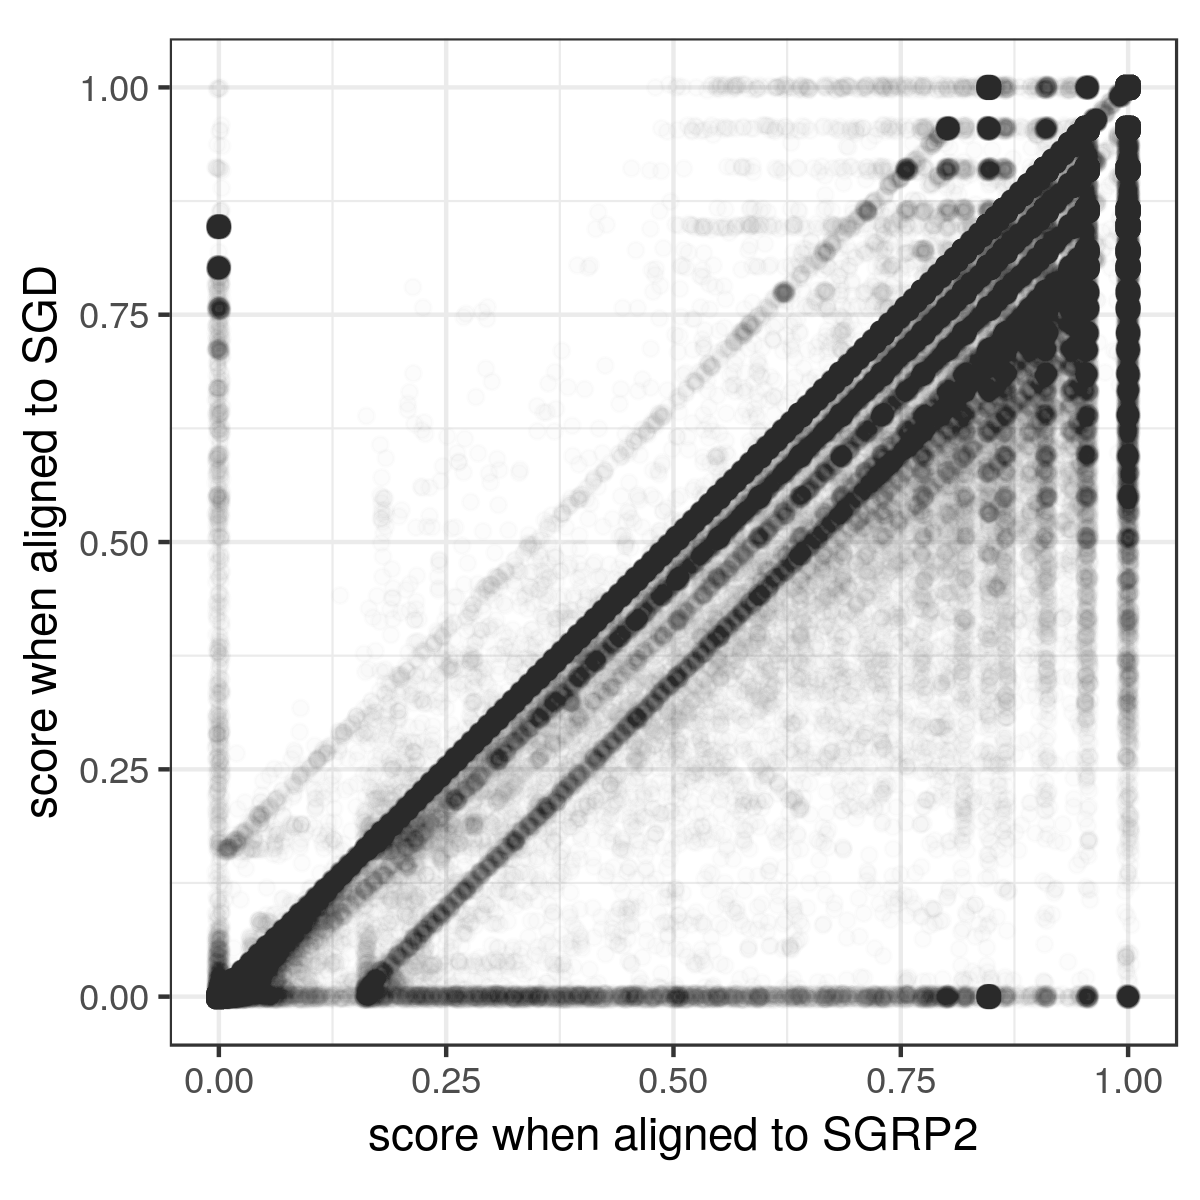
\includegraphics[width=1.0\textwidth]{Chapter3/Figs/NCYC_SGRP2_SGD_comparison_score.png}
    \caption{Alignment score} \label{subfig:NCYC_score}
  \end{subfigure}
  \begin{subfigure}[t]{0.49\textwidth}
    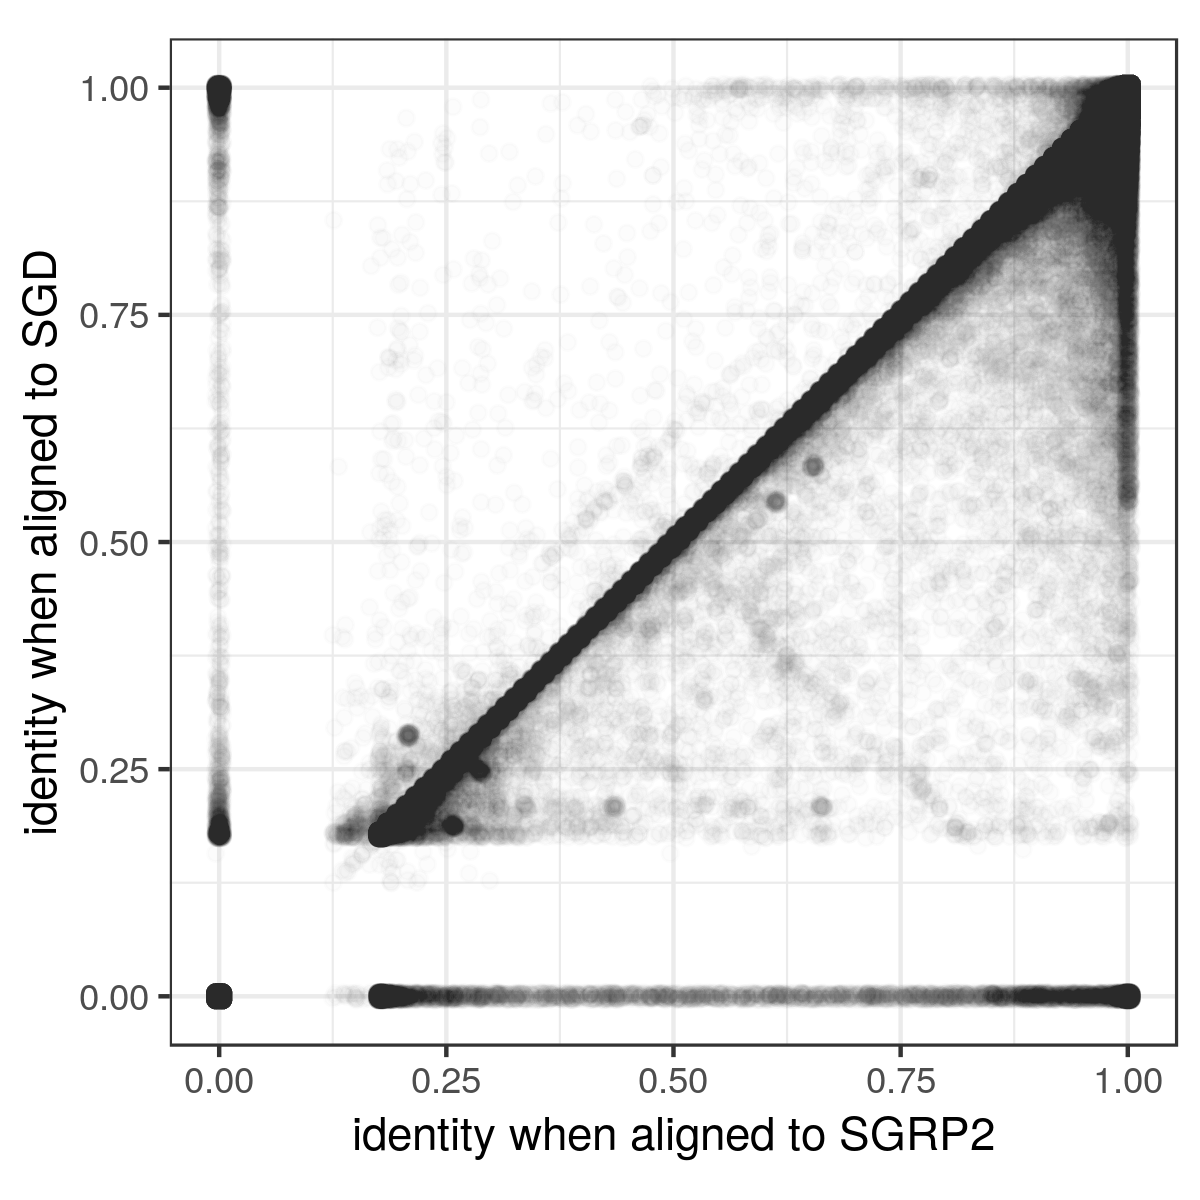
\includegraphics[width=1.0\textwidth]{Chapter3/Figs/NCYC_SGRP2_SGD_comparison_id.png}
    \caption{Alignment identity} \label{subfig:NCYC_identity}
  \end{subfigure}
  \begin{subfigure}[t]{1.0\textwidth}
    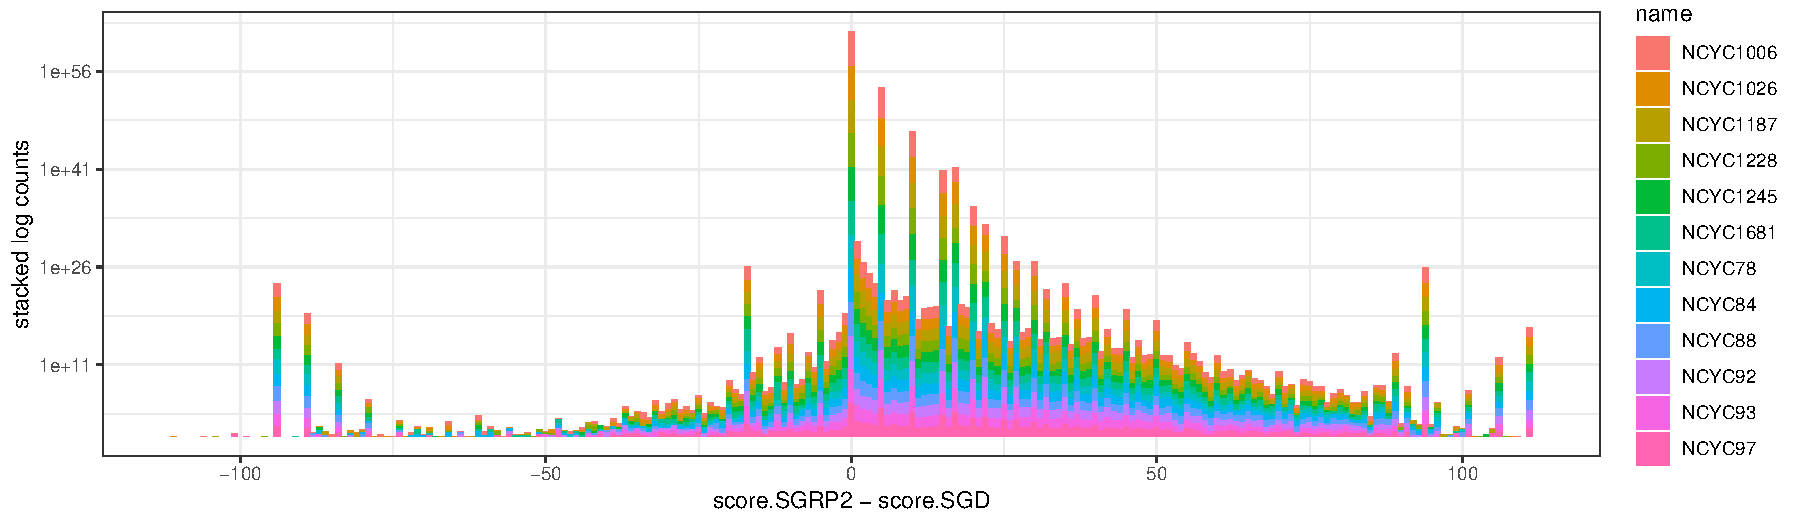
\includegraphics[width=1.0\textwidth]{Chapter3/Figs/NCYC_SGRP2_SGD_comparison_score_hist_color.pdf}
    \caption{Difference in alignment score} \label{subfig:NCYC_score_diff_hist}
  \end{subfigure}
  \begin{subfigure}[t]{1.0\textwidth}
    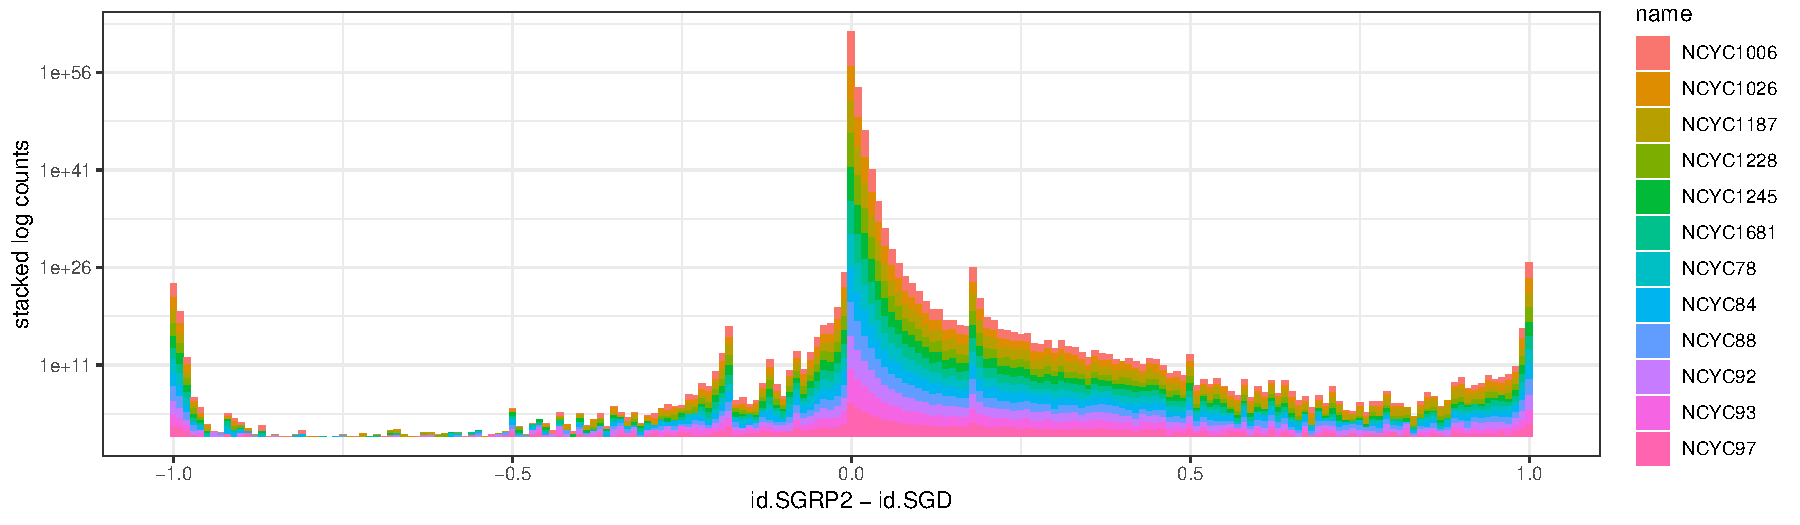
\includegraphics[width=1.0\textwidth]{Chapter3/Figs/NCYC_SGRP2_SGD_comparison_id_hist_color.pdf}
    \caption{Difference in alignment identity} \label{subfig:NCYC_id_diff_hist}
  \end{subfigure}
  \caption[Comparing alignment to the linear reference and SGRP2]{
    Alignment of 100k read pairs from 12 NCYC \emph{S. cerevisiae} strains(NCYC1006, NCYC1026, NCYC1187, NCYC1228, NCYC1245, NCYC1681, NCYC78, NCYC84, NCYC88, NCYC92, NCYC93, NCYC97) against the SGD\_2010 reference genome (SGD) or the SGRP2 pangenome (SGRP2).
    In (\ref{subfig:NCYC_score}) alignment scores are plotted for each read.
    The shift in density to the right relative to $y=x$ indicates improved alignments to the pangenome.
    In (\ref{subfig:NCYC_identity}) we observe the same pattern when using identity, or the fraction of the alignment which exactly matches the reference system.
    Subfigures \ref{subfig:NCYC_score_diff_hist} and \ref{subfig:NCYC_id_diff_hist} provide a log-scaled histogram of the difference in score and identity between the two graphs.
  }
\label{fig:NCYC_SGD_SGRP2}
\end{figure}

\subsection{Cactus progressive assembly}
%*0.5p 0.5h*
\label{sec:yeast_cactus}

Variation graphs are generic objects capable of representing any kind of alignment between genomes or assembly of read data from them.
To test the ability of {\tt vg} to use graphs of complex topology, we constructed a whole genome alignment graph of \emph{de novo} assemblies produced from Pacbio sequencing of seven strains of \emph{S. cerevisiae}.
In this assembly each chromosome of each assembly in \cite{yue2017contrasting} was progressively aligned using the phylogenetic guide tree methodology implemented in Cactus \cite{Paten:2011fva}.
As illustrated in figure \ref{fig:cactus_yeast_zoom}, this graph encodes a complex global topology that captures the structural variation between the species also reported in \cite{yue2017contrasting} as well as a local DAG-like topology which we expect when homologous sequences are represented compactly in a graph.
This illustrates the ability of vg to represent paths corresponding to both colinear (inset) and structurally rearranged (main figure) regions of genomic variation.

\begin{figure}[htbp!]
  \centering
  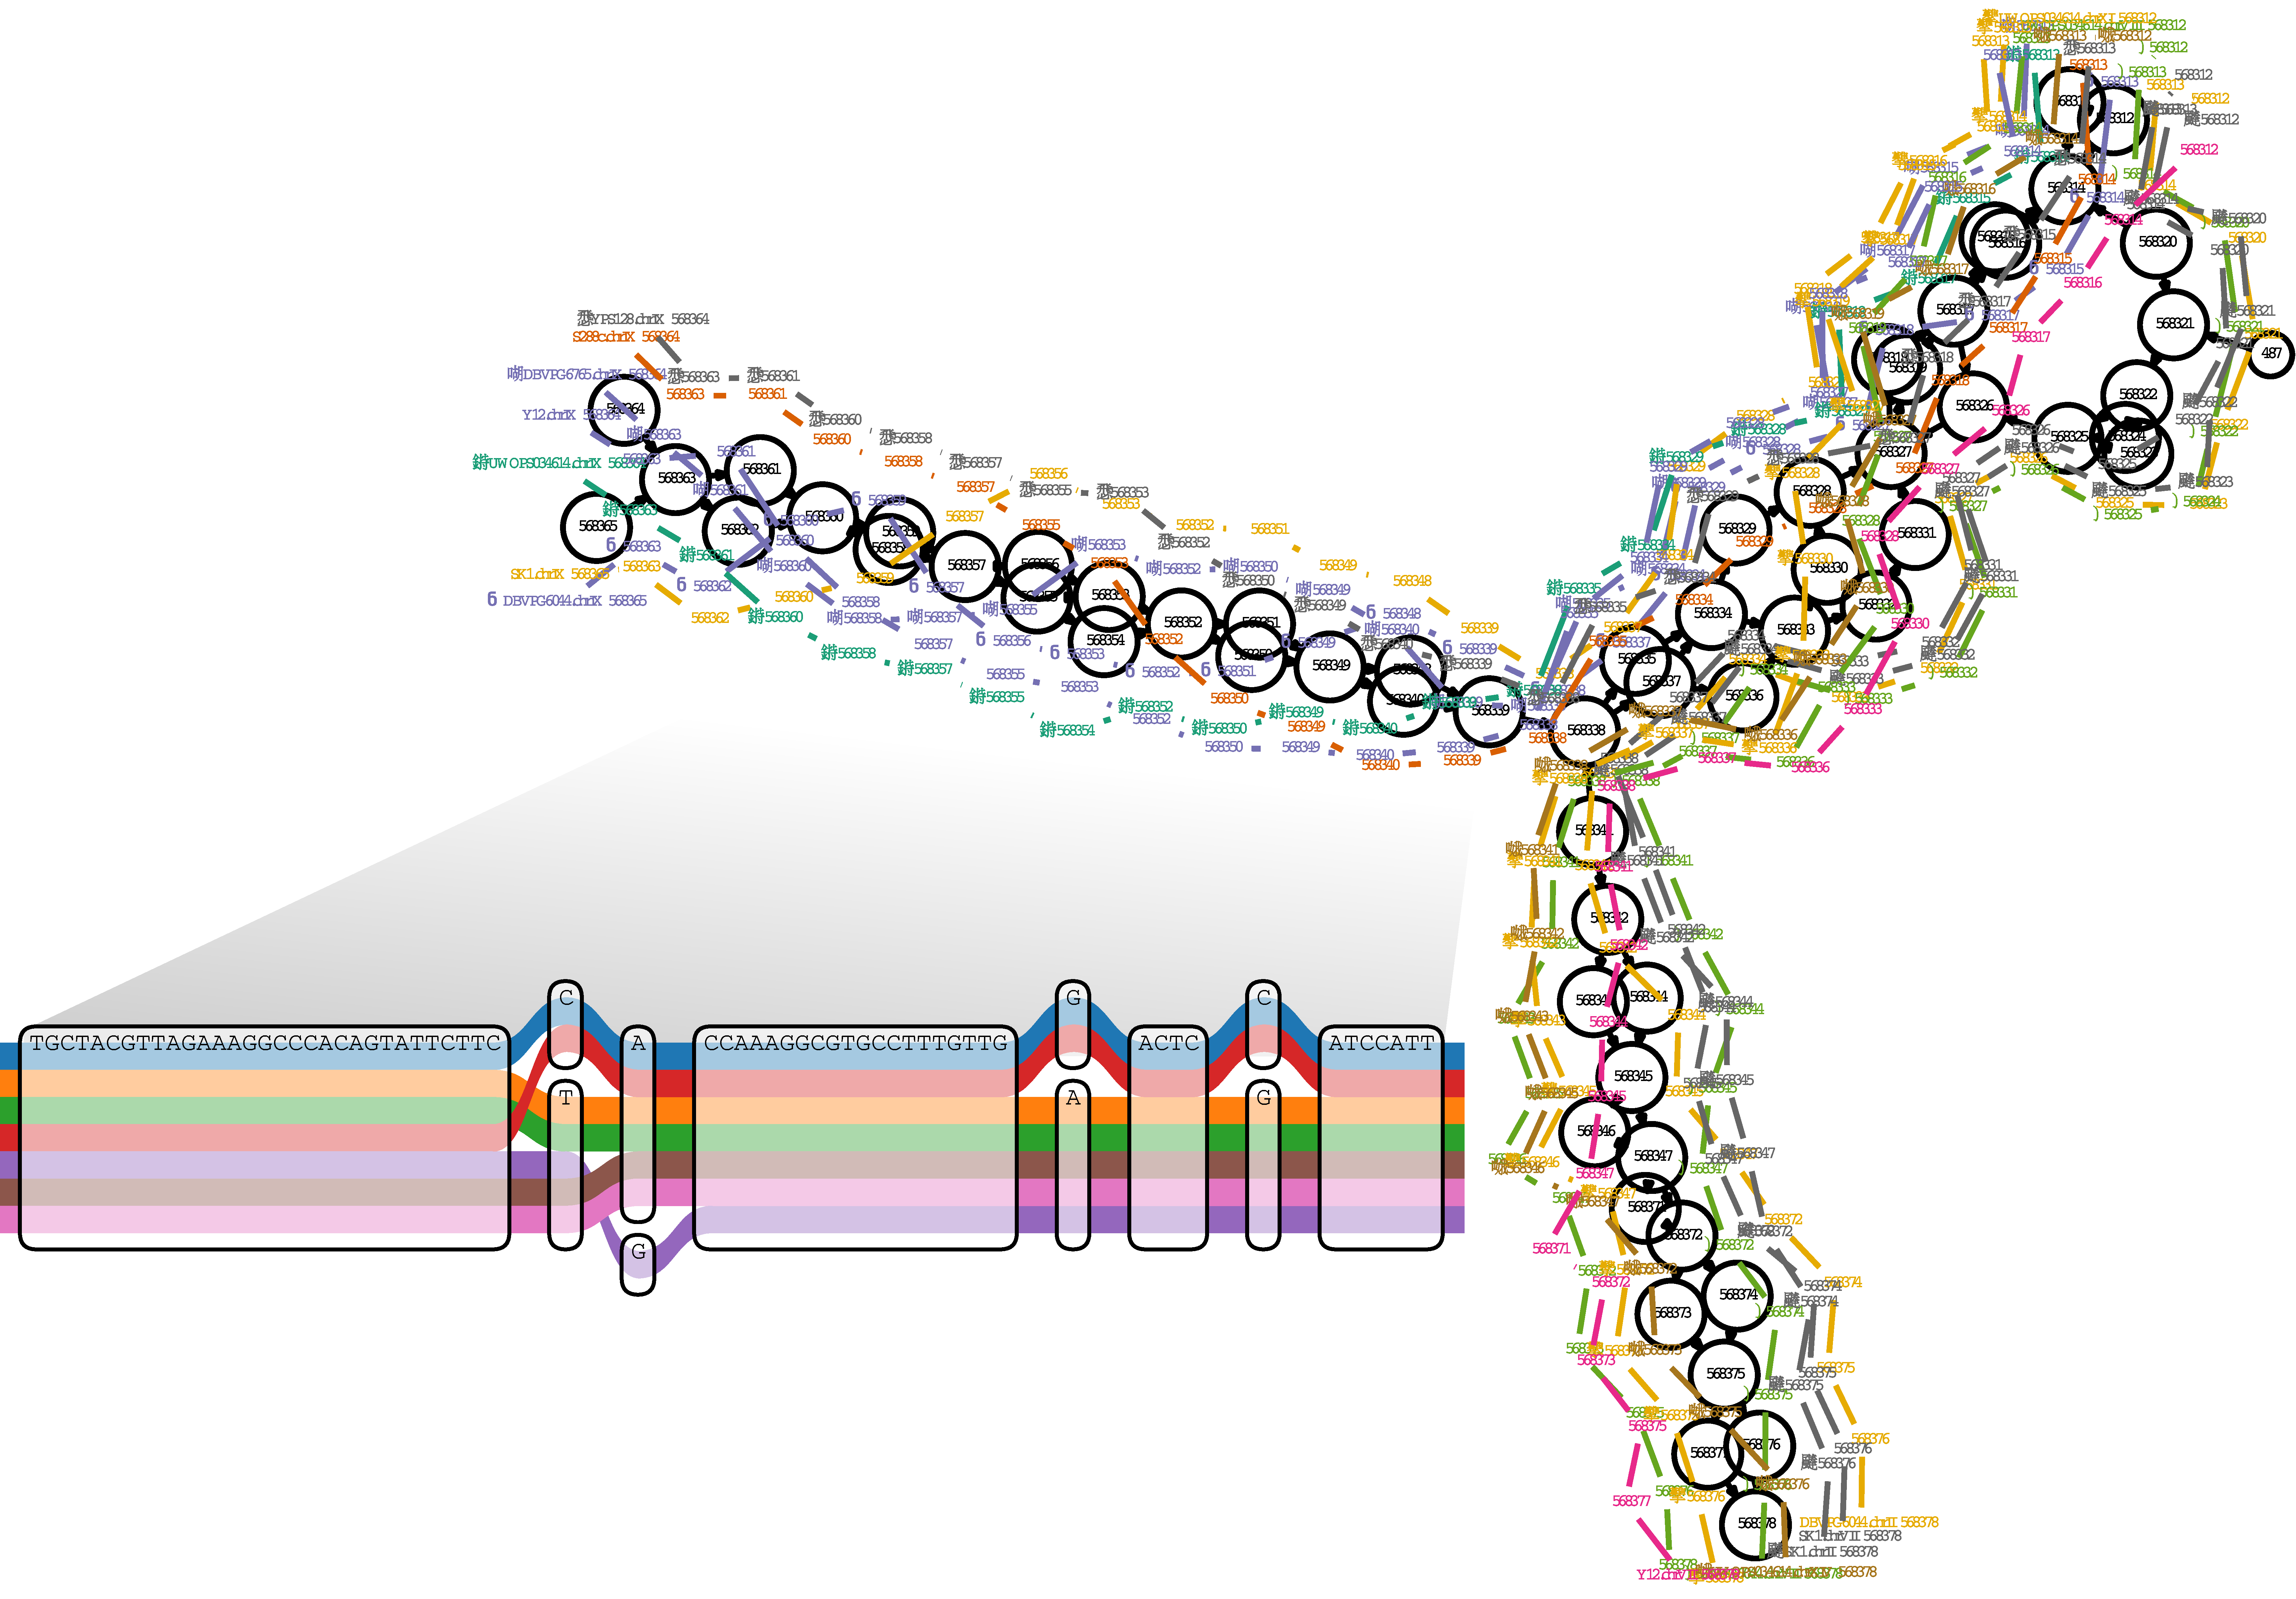
\includegraphics[width=1.0\textwidth]{Chapter3/Figs/cactus_yeast_zoom.pdf}
  \caption[Cactus yeast variation graph]{
  A region of a yeast genome variation graph.
  This displays the start of the subtelomeric region on the left arm of chromosome 9 in a multiple alignment of the strains sequenced in \cite{yue2017contrasting} as assembled by Cactus \cite{Paten:2011fva}.
  The inset shows a subregion of the alignment at single-base level.
  The colored paths correspond to separate contiguous chromosomal segments of these strains.
  }
  \label{fig:cactus_yeast_zoom}
\end{figure}

A simulation study based on the SK1 strain provides some insight into the capabilities of {\tt vg} and tradeoffs inherent in different graph designs.
I compared four vg graphs: a linear reference graph from the standard S288c strain, a linear reference from the SK1 strain, a pangenome graph of all seven strains, and a ``drop SK1'' variation graph in which all sequence private to the strain SK1 was removed from the pangenome graph.
The multiple genome graphs were constructed with the Cactus progressive aligner, which generates graphs that typically contain cycles and are not partially ordered, and then filtered down to the various subgraphs using path subsetting facilities in {\tt vg mod}.

\begin{figure}[htbp!]
  \centering
  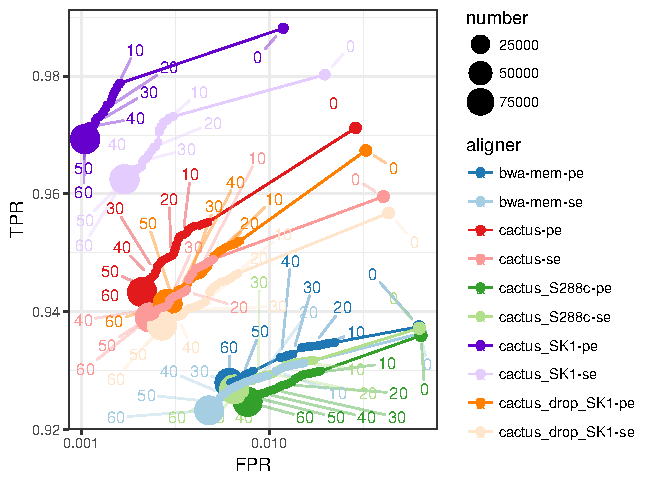
\includegraphics[width=0.65\textwidth]{Chapter3/Figs/e68fc338_test_sim_yeast_cactus-roc.pdf}
  \caption[Cactus yeast simulation]{Mapping short reads with vg to yeast genome references.
    ROC curves obtained by mapping 100,000 simulated SK1 yeast strain 150-bp paired-end reads against a variety of references described in the text.}
  \label{fig:cactus_yeast_sim}
\end{figure}


Similarly to the human experiments, we simulated 100,000 150-bp paired-end reads from the SK1 reference, modeling sequencing errors, and mapped them to the four references (ROC curves, Figure \ref{fig:cactus_yeast_sim}).
Not surprisingly, the best performance was obtained by mapping to a linear reference of the SK1 strain from which the data were simulated, with substantially higher sensitivity and specificity compared to mapping to the standard linear reference from the strain S288c with either {\tt vg} or {\tt bwa mem}.
Mapping to the variation graphs gave intermediate performance, with >1\% more sensitivity and lower false-positive rates than mapping to the standard reference.
There was surprisingly little difference between mapping to graphs with and without the SK1 private variation, probably because much of what is novel in SK1 compared to the reference is also seen in other strains.
We saw lower sensitivity compared to mapping just to the SK1 sequence, likely because of suppression of GCSA2 index $k$-mers in complex or duplicated regions, which our indexing strategy was not designed to address.

\subsection{Constructing diverse \emph{cerevisiae} variation graphs}
\label{sec:constructing_yeast_graphs}

With {\tt vg}, our goal is to build a toolkit that allows the use of any genome graph as a reference.
To validate this capability, I used data sources for \emph{S. cerevisiae} to build seven variation graphs, whose dimensions are listed in table \ref{table:yeast_graphs}.
In the next section (\ref{sec:yeast_long_read}) I present an evaluation of these graphs using long reads from the SK1 strain.


\begin{table}[h]
  \centering
\begin{tabular}{l||c|c|c|c|c}
\itshape name & \itshape size (MB) & \itshape length & \itshape nodes & \itshape edges & \itshape subgraphs \\
\hline
SGD\_2010 & 7.3 & 12163423 & 380115 & 380097 & 18 \\
S288c & 7.3 & 12249246 & 382797 & 382781 & 18 \\
SGRP2 & 21 & 12407052 & 714533 & 969690 & 18 \\
minia unitigs & 15 & 14419206 & 1232804 & 1332994 & 46131 \\
minia contigs & 6.4 & 12233279 & 421125 & 425683 & 2961 \\
Cactus & 31 & 13243056 & 1059173 & 1304205 & 580 \\
{\tt vg msga} & 42 & 13793955 & 1156295 & 1387903 & 2 \\
\hline
\end{tabular}
\caption{A summary of seven different variation graphs contructed to represent variation in \emph{S. cerevisiae}.
  As described in section \ref{sec:SGRP2_graph}, the SGD\_2010 graph is built from the reference, while SGRP2 adds SNPs in the SGRP2 population survey.
  The Illumina data from \cite{yue2017contrasting} was used to build the minia unitigs and minia contigs graphs, while the whole genome, chromosome-resolved PacBio assemblies from the same work were used to build the Cactus and {\tt vg msga} progressive assemblies.
  S288c is the \emph{de novo} assembly of the reference strain produced in \cite{yue2017contrasting}.
}
\label{table:yeast_graphs}
\end{table}

Three of the graphs are effectively linear or DAG-like, with the exception of their mitochondria and plasmid chromosomes, which are included as circular components.
SGD\_2010 and S288c represent two assemblies of the reference genome, the former from the SGD genome sequencing project, and the latter is a \emph{de novo} assembly from \cite{yue2017contrasting}.
The difference in quality between the two approaches will be made apparent in the subsequent section.
As described in section \ref{sec:SGRP2_graph}, the SGRP2 graph adds SNP variation from the population survey in \cite{bergstrom2014high} to build a pangenome reference.
The SGD\_2010 reference contains the mitochondria and 6kb plasmid sequence, while the S288c assembly excludes them due to the sequencing protocol, where size selection in the library preparation stage removed these short sequences, so to enable direct comparison in later tests these were added to the S288c graph.

The remaining four graphs are different forms of assembly graph.
Using the Illumina data published in \cite{yue2017contrasting}, I build two assemblies with minia3, using a $k$-mer size of 51 and a high abundance threshold (50) to limit the resulting graph complexity.
In the first, I take the unitig graph that represents all non-branching paths in the compacted DBG as nodes.
The second is the result of the minia contigification process that pops bubbles and cleans the graph to attempt to arrive at longer contigs.
Both results are expressed as overlap graphs in GFA, and I can import them as variation graphs using bluntification and graph pseudotopological sorting.
As shown in table \ref{table:yeast_graphs}, the unitig graph is considerably more complex in terms of node density than the contig graph.
It also contains more sequence, presumably because some regions that are collapsed in the contig graph are not in the unitig graph.
The number of disjoint components in these graphs is very high (2961 for the contig graph and 46131 for the unitig graph), suggesting that pruning of the assembly graph has yielded a greatly fragmented result.
The resulting graphs are difficult to align long reads to.
I conclude that further tuning of the paramaters used during \emph{de novo} assembly from short reads will be required to use assemblies like this as reference graph.

Finally, I used the whole genome \emph{de novo} assemblies of long read data from \cite{yue2017contrasting} to build whole genome alignment graphs using Cactus (as described in section \ref{sec:yeast_cactus}) and {\tt vg msga}.
The multiple sequence to graph alignment (MSGA) process implemented in {\tt vg msga} is akin to the progressive POA method, but generalized to arbitrary graphs of any size.
Rather than using a local alignment algorithm to expand the graph, the long read alignment algorithm described in section \ref{sec:chunked_alignment} allows the direct alignment of whole chromosomes to the graph.
Where the Cactus progressive assembly uses a phylogenetic guide tree to sturcture its construction, {\tt vg msga} simply aligns the chromosomes in order from longest to shortest to the growing graph.
The long read alignment in {\tt vg} is structured to enforce long range synteny, and the resulting graph is substantially different in sturcture than that of Cactus.
I find that {\tt vg msga} is less likely to collapse repeats than Cactus, at least in the configuration used for this assembly.
We can see this in figure \ref{fig:yeast_bandage}, where the Cactus graph (\ref{subfig:cactus_yeast_bandage}) shows two dense repeat structures in its core connected by loops of unique sequence, while the {\tt vg msga} graph appears to have much longer loops, with collapsed repeats embedded in these loops.
This observation is supported by the length statistics in table \ref{table:yeast_graphs}, with {\tt vg msga} producing a graph that is 550,899bp longer than that of Cactus.
At the same time, the node count of the {\tt vg msga} graph is higher, which perhaps reflects a different local alignment result.

\begin{figure}[htbp!]
  \begin{subfigure}[t]{0.9\textwidth}
    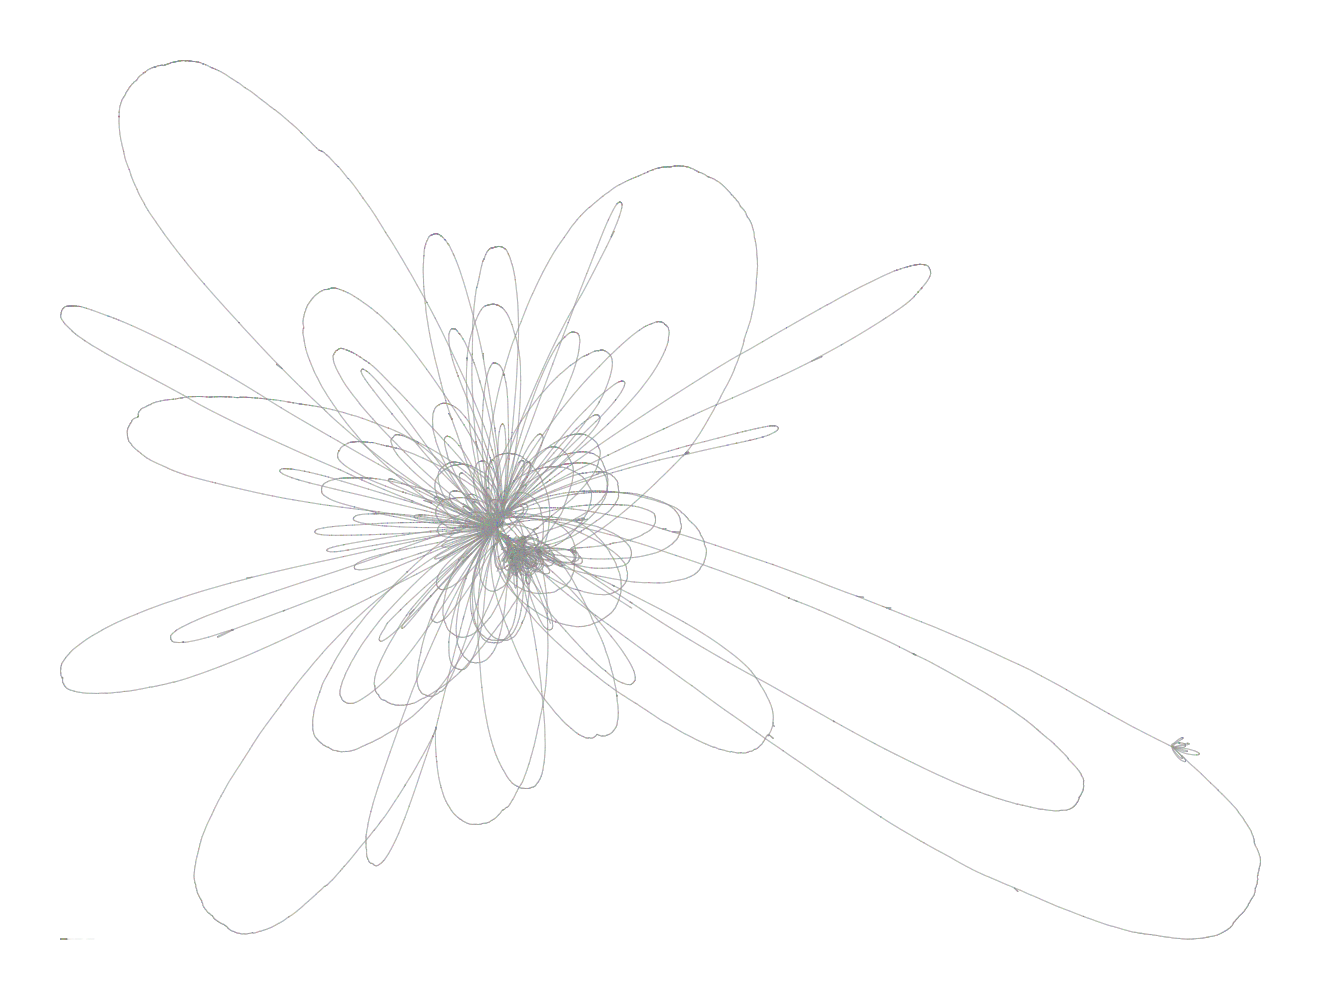
\includegraphics[width=1.0\textwidth]{Chapter3/Figs/cactus_yeast.png}
    \caption{Cactus assembly} \label{subfig:cactus_yeast_bandage}
  \end{subfigure}
  \begin{subfigure}[t]{0.9\textwidth}
    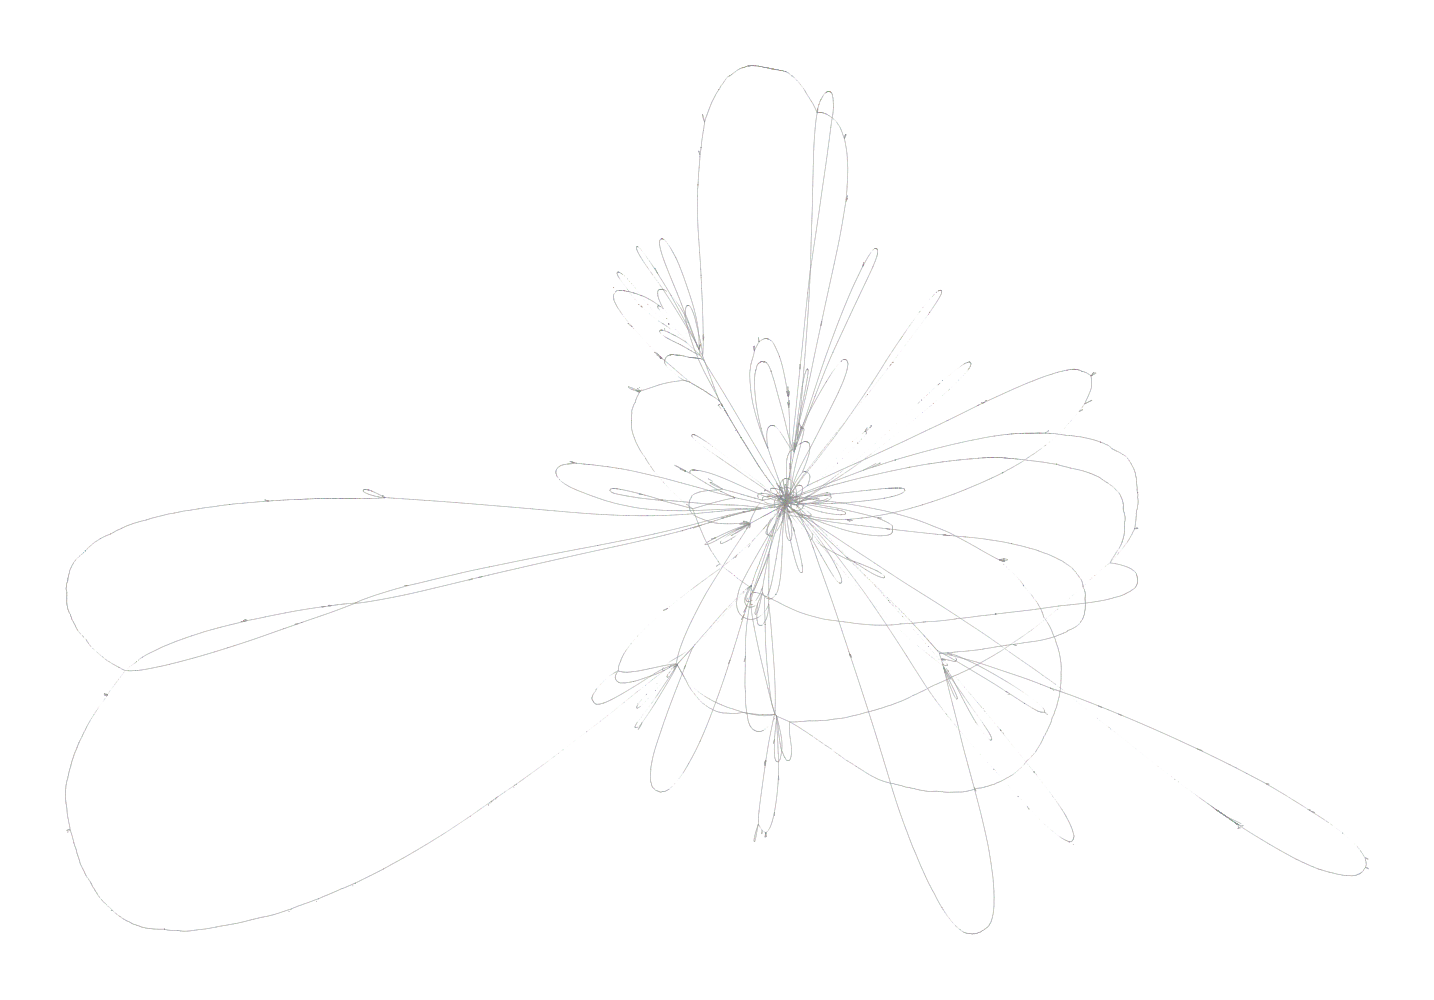
\includegraphics[width=1.0\textwidth]{Chapter3/Figs/vg_msga_yeast.png}
    \caption{{\tt vg msga} assembly} \label{subfig:msga_yeast_bandage}
  \end{subfigure}
  \caption[Whole genome alignment graphs for \emph{S. cerevisiae}]{
    Whole genome alignment graphs for \emph{S. cerevisiae} visualized using Bandage.
    The scale in \ref{subfig:msga_yeast_bandage} is greater than that in \ref{subfig:cactus_yeast_bandage}, with the latter showing a greater propensity to collapse repeat structures.
  }
  \label{fig:yeast_bandage}
\end{figure}

\subsection{Using long read mapping to evaluate \emph{cerevisiae} graphs} % from paper / my experiments
\label{sec:yeast_long_read}

In this section I evaluate the graphs I constructed in section \ref{sec:constructing_yeast_graphs} and simultaneously demonstrate the ability of {\tt vg} to align long reads to graphs of any type.
For each of the seven graphs I aligned a set of 43,337 Pacific Biosciences SK1 reads (mean length 4.7 kb) from \cite{yue2017contrasting} to the graph.
We can then compare the alignment identity for each read across the various graphs.
I do so using the same dot plot techinque used to demonstrate alignment quality improvement using the Illumina data from the NCYC strains.
In figure \ref{fig:pacbio_yeast} I present a number of pairwise comparisons based on this read set.

I find that the SGD\_2010 reference provides a better match for the SK1 PacBio reads than the S288c assembly (top left), which can be seen in a subset of reads that map nearly perfectly to the SGD\_2010 graph but not to the S288c one.
This may be due to the higher quality and curation of the SGD reference, which was initially based on BACs and capillary sequencing, but I have not determined the exact cause of this discrepancy.
This same effect is clear in the comparison of S288c and the SGRP2 (top middle, figure \ref{fig:pacbio_yeast}), although there the SNPs in the SGRP2 graph tend to improve the overall match between the SK1 reads and the graph, which can be seen in a shift in density upwards from the diagonal.
For other comparisons I focused on using the S288c reference, as it forms a part of the progressive alignments and the source data for the minia assemblies comes from the same paper.

The minia graphs appear to provide very low quality as a reference for the alignment of long reads (bottom left and middle, figure \ref{fig:pacbio_yeast}).
The minia unitig graph is too fragmented for any practical use.
In almost no case does it provide a better a better match for the long reads.
However, while the minia contig graph is also outperformed by the S288c graph, for a notable subset of the reads it provides a perfect match, while the S288c graph fails to match them at all.
This suggests that some contigs in the Illumina assembly match the SK1 strain, which is to be expected and demonstrates that in principle this kind of graph can represent multiple genomes.

Finally, the whole genome alignment graphs are notable in their similarity.
Despite the fact that they were constructed using different algorithms, both provide a similar basis for alignment of the SK1 reads.
It is notable that alignment time against the {\tt vg msga} graph was the highest of any of the tested graphs, and significantly higher than that for the Cactus graph.
This may relate to the un-collapsed state of the repeats in the graph.
The alignment algorithm will attempt more alignments for each band where there is ambiguity, and the ``patching'' at the end of the alignment process will be more intensive.

\begin{figure}[htbp!]
  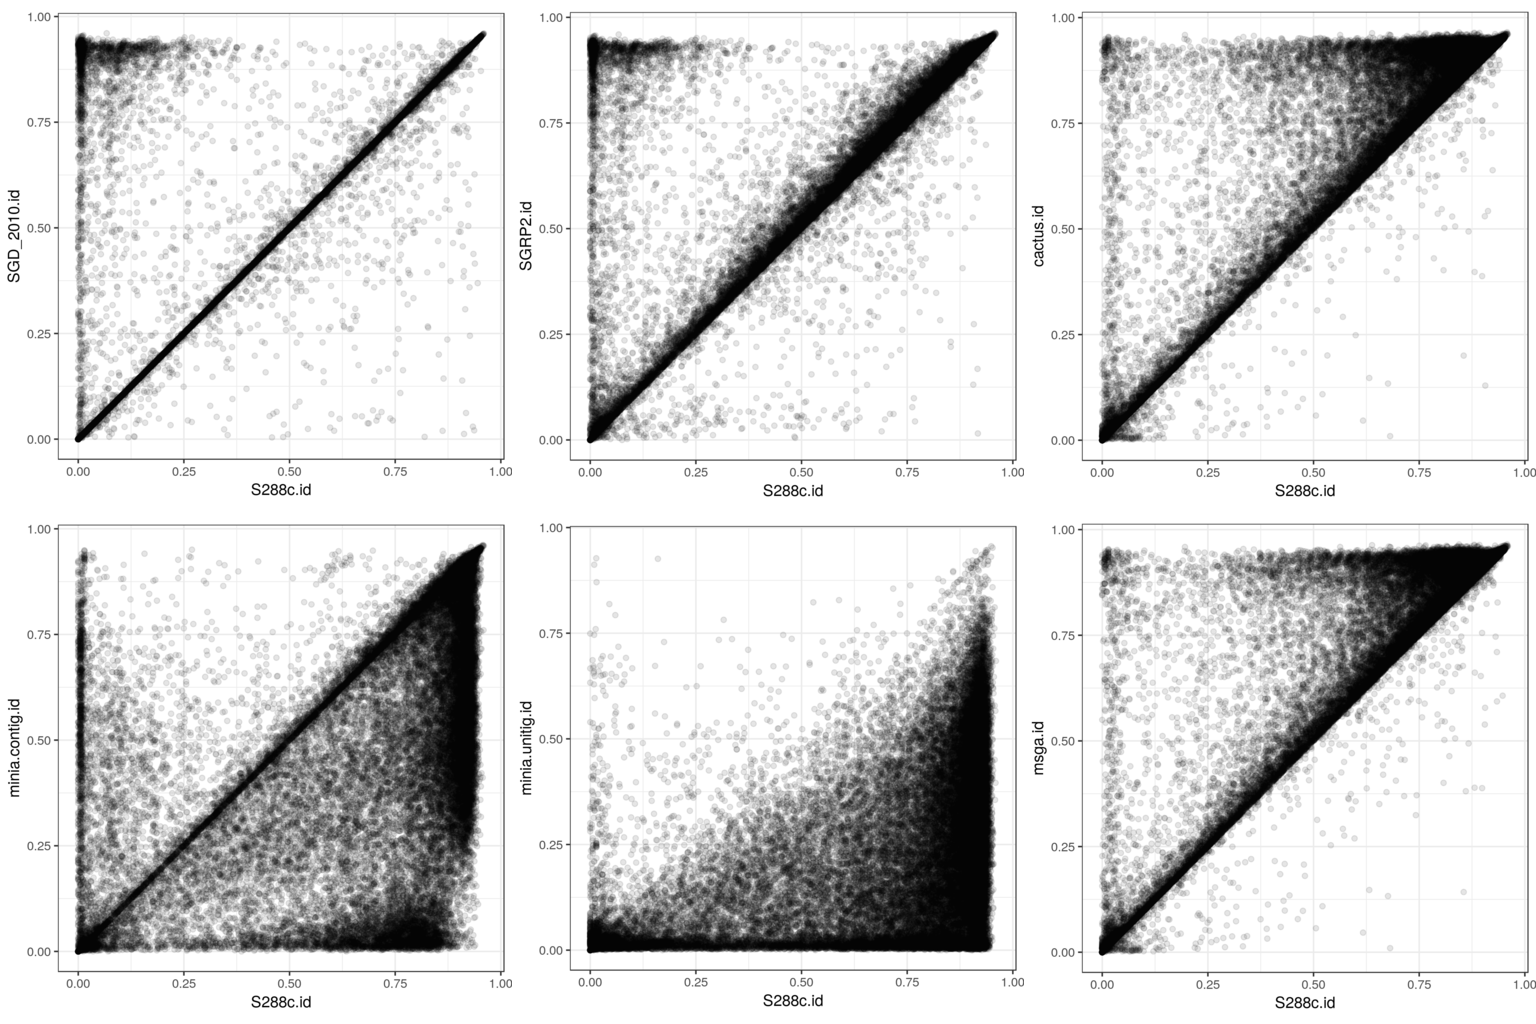
\includegraphics[width=1.0\textwidth]{Chapter3/Figs/montage_vs_S288c_3x2.png}
  \caption[Long read alignment against various \emph{S. cerevisiae} pangenome graphs]{Density plots of alignment identity when mapping 43,337 Pacific Biosciences long reads from the SK1 strain to different variation graphs.
    \emph{Linear assemblies}:
    (Top left) the SGD\_2010 reference vs. the S288c assembly from \cite{yue2017contrasting}.
    (Top middle) the S288c assembly vs. the SGRP2 SNP pangenome.
    \emph{Assembly graphs from Illumina data}:
    (Bottom left) the minia contig graph vs. the S288c assembly.
    (Bottom middle) the minia unitig graph vs. the S288c assembly.
    \emph{Whole genome alignment graphs}:
    (Top right) the Cactus alignment vs. the S288c assembly.
    (Bottom right) the {\tt vg msga} alignment vs. the S288c assembly.
  }
  \label{fig:pacbio_yeast}
\end{figure}


\section{Human}
%*0.5p 0.5h*

For a species such as human, with only 0.1\% nucleotide divergence on average between individual genome sequences, over 90\% of 100-bp reads will derive from sequence exactly matching the reference.
Therefore, new mappers should perform at least as well for linear reference mapping as the current standard, which we take to be {\tt bwa mem} with default parameters.
We show that vg does this, and then that vg maps more informatively around divergent sites.

\subsection{1000GP graph construction and indexing}
%*3p 3h*

The final phase of the 1000 Genomes Project (1000GP) produced a data set of ~80 million variants in 2,504 humans 16.
We made a series of vg graphs containing all variants or those with minor allele frequency thresholds at 0.1\%, 1\%, or 10\%, as well as a graph corresponding to the standard GRCh37 linear reference sequence without any variation.
The full vg graph uses 3.92 GB when serialized to disk, and contains 3.181 Gbp of sequence, which is exactly equivalent to the length of the input reference plus the length of the novel alleles in the VCF file.
Complete file sizes including indices range from 25 GB to 63 GB, with details including build and mapping times given in table \ref{table:1000GP}.

\begin{table}[h]
\begin{tabular}{l||c|cc|cc|cc}
\itshape Reference set & \itshape N vars & \multicolumn{2}{c}{\itshape vg} & \multicolumn{2}{c}{\itshape index} & \multicolumn{2}{c}{\itshape search time}\\
& \itshape (M) & \itshape time & \itshape size & \itshape time & \itshape size & \itshape  PE & \itshape SE\\
\hline
GRCh37 & 0 & 1:09:54 & 1.76 & 23:30:41 & 25.11 & 33:34 & 28:33 \\
1000GP AF0 & 84.8 & 3:42:01 & 3.92 & 51:05:07 & 63.28 & 45:10 & 39:46 \\
1000GP AF0.001 & 30.2 & 2:00:08 & 2.58 & 31:45:12 & 38.10 & 39:33 & 32:53 \\
1000GP AF0.01 & 14.3 & 1:35:02 & 2.17 & 27:18:53 & 30.94 & 33:13 & 27:09\\
1000GP AF0.1 & 6.8 & 1:23:04 & 1.97 & 26:06:38 & 27.79 & 32:35 & 28:43 \\
\hline
\end{tabular}
\caption{Numbers of variants, file sizes in gigabytes (GB) and build and search times in hours:minutes:seconds for various human vg graphs and associated indexes. Reference sets are the linear reference GRCh37, the full 1000 Genomes Project set 1000GP AF0, and subsets of 1000GP AF0 including only variants with allele frequency above thresholds 0.001 (0.1\%), 0.01 (1\%) and 0.1 (10\%) respectively.  The number of variants in millions for each of these data sets is shown.  Search times are for 10 million 150+150bp read pairs simulated from NA24385.
}
\label{table:1000GP}
\end{table}

\subsection{Simulations based on phased HG002}
\label{sec:1000GP_sim}

We next aligned ten million 150-bp paired-end reads simulated with errors from the parentally phased haplotypes of an Ashkenazi Jewish male NA24385, sequenced by the Genome in a Bottle (GIAB) Consortium \cite{zook2016extensive} and not included in the 1000GP sample set, to each of these graphs as well as to the linear reference using {\tt bwa mem}.
Figure \ref{fig:HG002_1000GP_sim} shows the accuracy of these alignments compared with {\tt bwa mem} for the the full range of frequency thresholded graph, in terms of receiver operating characteristic (ROC) curves.

Reads that come from parts of the sequence without differences from the reference (middle panels of Figure \ref{fig:HG002_1000GP_sim}) mapped slightly better to the reference sequence (green) than to the 1000GP graph (red), which we attribute to a combination of the increase in options for alternative places to map reads provided by the variation graph, and the fact that we needed to prune some search index $k$-mers in the most complex regions of the graph.
The best balance of performance appears at the threshold of 0.01, as in panel C.
As expected, this difference increased as the allele frequency threshold was lowered and more variants were included in the graph, as seen in Figure \ref{fig:HG002_1000GP_sim} panels A and B.

For reads that were simulated from segments containing non-reference alleles (~10\% of reads), which are the reads relevant to variant calling, {\tt vg} mapping to the 1000GP graph (red) gave better performance than either {\tt vg} (green) or {\tt bwa mem} (blue) mapping to the linear reference (right panels of Figure \ref{fig:HG002_1000GP_sim}), because many variants present in NA24385 are already represented in the 1000GP graph.
This is particularly clear for single-end mapping, since many paired-end reads are rescued by the mate read mapping.
Overall, vg performed at least as well as bwa mem, even on reference-derived reads, and substantially better on reads containing non-reference variants.

\begin{figure}[htbp!] 
\centering    
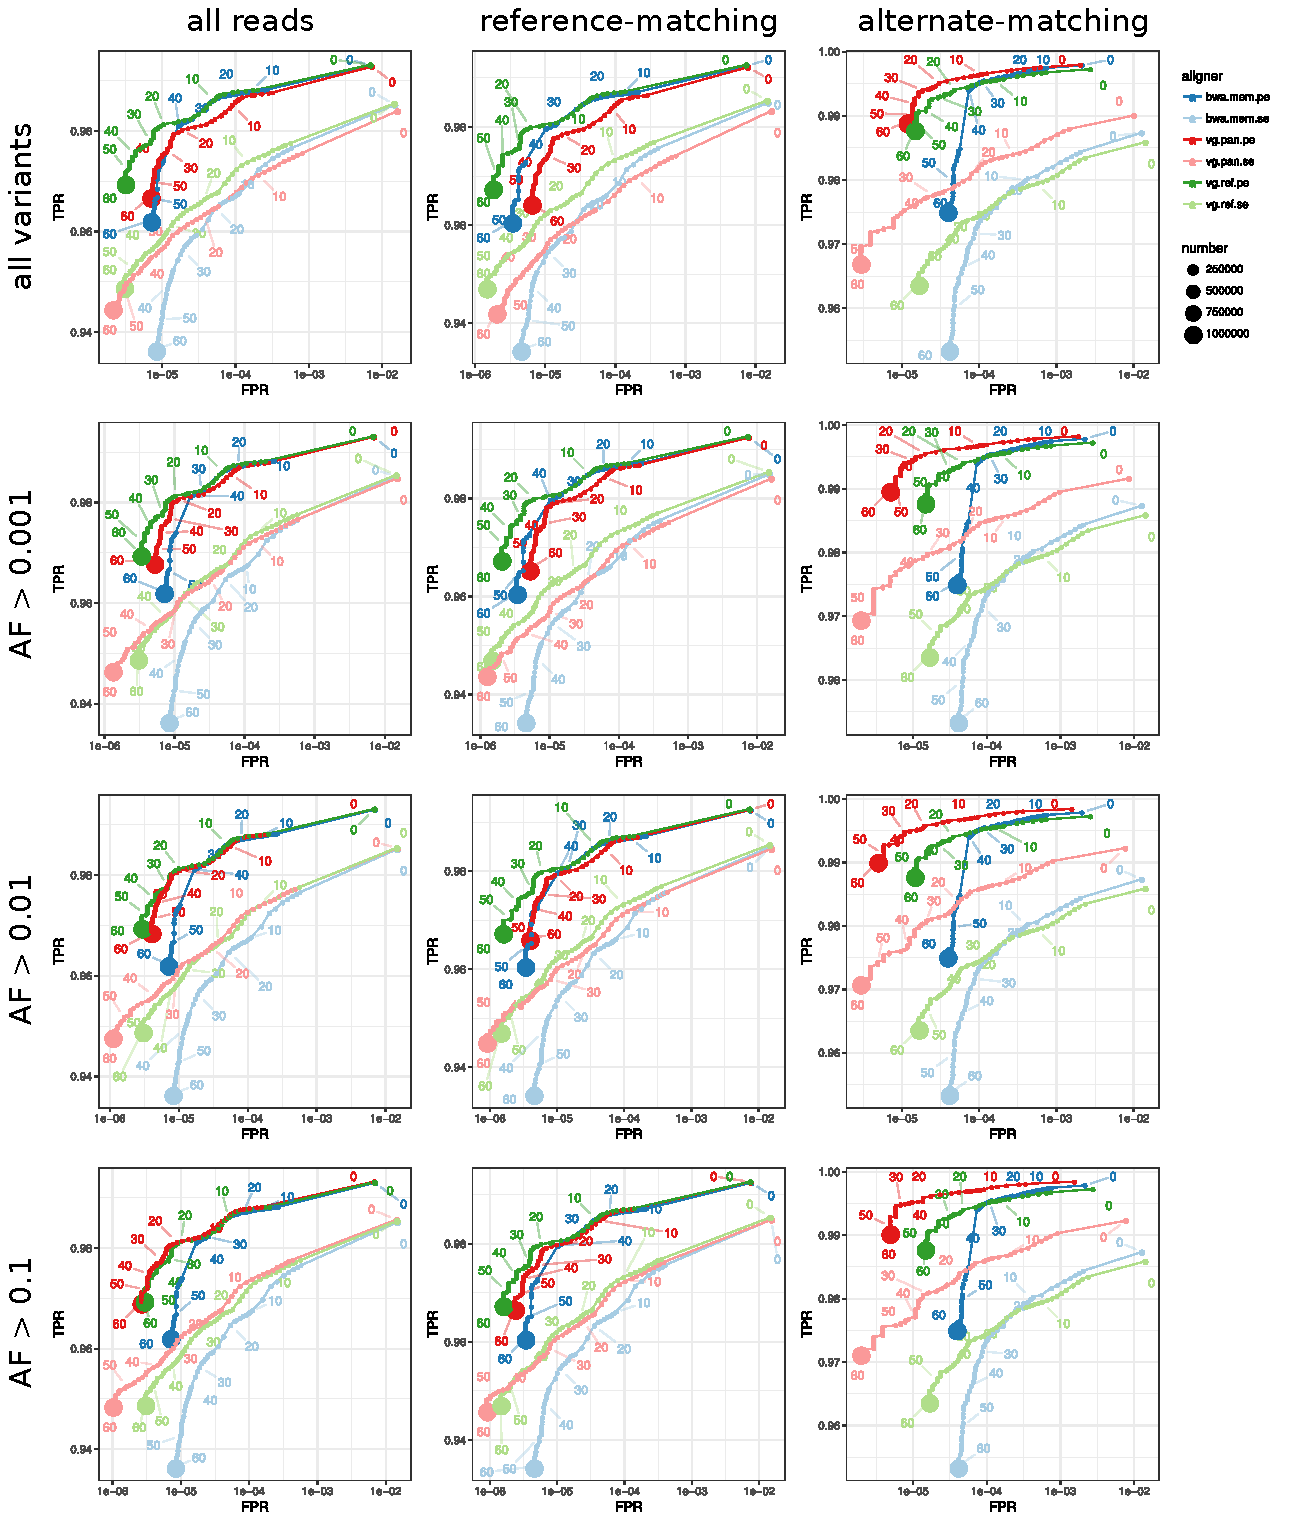
\includegraphics[width=1.0\textwidth]{Chapter3/Figs/human-10M-results-7358a67_merge_panel_labeled.pdf}
\caption[Simulated reads from HG002 versus various human pangenome graphs.]{
  ROC curves parameterised by mapping quality for 10M read pairs simulated from NA24385 as mapped by bwa mem, vg to various 1000GP pangenome references, and vg with a linear reference, using single end (se) or paired end (pe) mapping.
  Allele frequency thresholds for the various panels are A) all variants, B) 0.001, C) 0.01, and D) 0.1.
  Within each panel, the left subpanel is based on all reads, middle on reads simulated from segments with no genetic variants from the linear reference, right on reads simulated from segments containing variants.
  All reads may contain simulated sequencing errors reflecting SNPs at a rate of 0.01 per base and indels at a rate of 0.002 per base.}
\label{fig:HG002_1000GP_sim}
\end{figure}

\subsection{Aligning and analyzing a real genome}

We also mapped a real human genome read set with ~50× coverage of Illumina 150-bp paired-end reads from the NA24385 sample to the 1000GP graph. vg produced mappings for 98.7\% of the reads, 88.7\%
with reported mapping quality score 30 on the Phred scale, and 76.8\% with perfect, full-length sequence identity to the reported path on the graph.
For comparison, we also used vg to map these reads to the linear reference.
Similar proportions of reads mapped (98.7\%) and with reported quality score 30 (88.8\%), but considerably fewer with perfect identity (67.6\%).
Markedly different mappings were found for 1.0\% of reads (0.9\% mapping to widely separated positions on the two graphs, and 0.1\% mapping to one graph but not the other).
The reads mapping to widely separated positions were strongly enriched for repetitive DNA. For example, the linear reference mappings for 27.5\% of these read pairs overlapped various types of satellite DNA identified by RepeatMasker, compared to 3.0\% of all read pairs.

To illustrate the consequences of mapping to a reference graph rather than a linear reference, we stratified the sites independently called as heterozygous in NA24385 by deletion or insertion length (0 for single-nucleotide variants) and by whether the site was present in 1000GP, and measured the fraction of reads mapped to the alternate allele for each category.
The results show that mapping with vg to the population graph when the variant was present in 1000GP (95.4\% of sites) gave nearly balanced coverage of alternate and reference alleles independent of variant size, whereas mapping to the linear reference either with {\tt vg} or {\tt bwa mem} led to a progressively increasing bias with increasing deletion and (especially) insertion length (Figure \ref{fig:HG002_indels}), so that for insertions around 30 bp, a majority of insertions containing reads were missing (there were over twice as many reference reads as alternate reads).

\begin{figure}[htbp!] 
\centering    
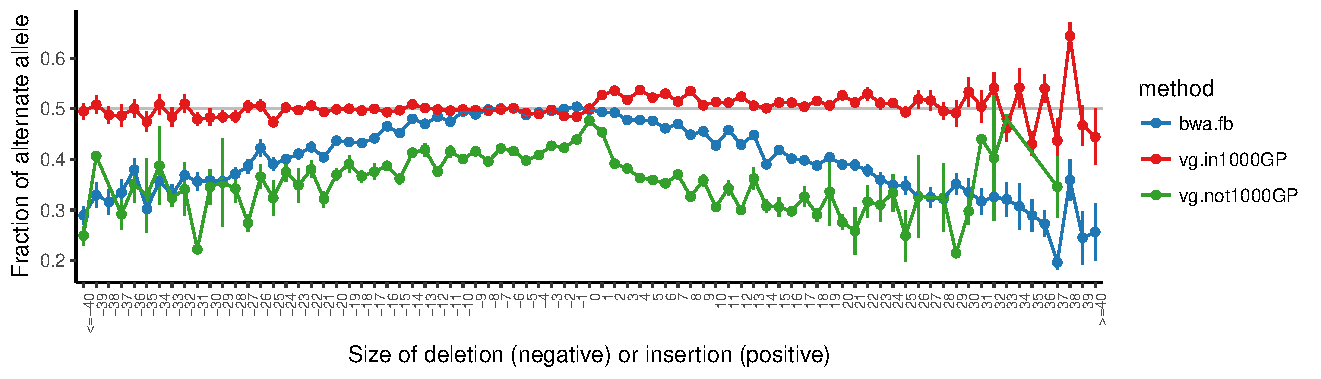
\includegraphics[width=1.0\textwidth]{Chapter3/Figs/HG002_wg_pan_ref_bwa_true_hets_allele_balance_tsv_gz_3.pdf}
\caption[Indel allele balance in HG002]{The mean alternate allele fraction at heterozygous variants previously called in HG002/NA24385 as a function of deletion or insertion size (SNPs at 0). Error bars are ± 1 s.e.m.}
\label{fig:HG002_indels}
\end{figure}

\subsection{Whole genome variant calling experiments}

We explored the application of {\tt vg} to whole genome alignment and variant calling in the PrecisionFDATruth Challenge, in which the team which developed the Genome in a Bottle truth set developed and held out a new sample.
Methods were first tested against publicly available truth sets on NA12878 in the ``consistency'' challenge, in which the {\tt vg} development team received a star for ``heroic effort'' in completing the first whole-genome graph based alignment and variant calling analysis.
The results for this first iteration were very poor, with F-scores for indels and SNPs around 95\%.
The computational costs were high, with the run consuming around \$1000 in resources on Amazon's Elastic Compute cloud (AWS EC2).

In the final round of the challenge, we obtained results as described in table \ref{table:PFDA}.
We find that the {\tt vg} pipeline had similar performance to the \emph{de novo} assembly pipeline fermikit for SNPs.
Methods that are not explicitly based on the GATK indel calling method perform notably worse on indels, including egarrison-hhga\footnote{This was my work along with Nicolas Della Penna, \url{https://github.com/ekg/hhga}. Unfortunately, it remains unpublished.}, which used Platypus, fermikit, and freebayes to generate candidate variants and implemented a genotyper using a machine learning method, and mlin-fermikit, which was a direct application of fermikit's standard pipeline to the data for HG002.
However, {\tt vg call}'s indel calling results were very poor, and likely caused by bugs in the variant caller and aligner at this stage rather than conceptual problems with graph based variant calling.

\begin{table}[h]
\begin{tabular}{l||ccc|ccc}
\itshape Submission & \multicolumn{3}{c}{\itshape SNPs} & \multicolumn{3}{c}{\itshape indels}\\
& \itshape F-score & \itshape recall & \itshape precision & \itshape F-score & \itshape recall & \itshape precision \\
\hline
anovak-vg & 98.4545 & 98.3357 & 98.5736 & 70.4960 & 69.7491 & 71.2591 \\
astatham-gatk & 99.5934 & 99.2091 & 99.9807 & 99.3424 & 99.2404 & 99.4446 \\
bgallagher-sentieon & 99.9296 & 99.9673 & 99.8919 & 99.2678 & 99.2143 & 99.3213 \\
dgrover-gatk & 99.9456 & 99.9631 & 99.9282 & 99.4009 & 99.3458 & 99.4561 \\
egarrison-hhga & 99.8985 & 99.8365 & 99.9607 & 97.4253 & 97.1646 & 97.6874 \\
hfeng-pmm3 & 99.9548 & 99.9339 & 99.9756 & 99.3628 & 99.0161 & 99.7120 \\
mlin-fermikit & 98.8629 & 98.2311 & 99.5029 & 95.5997 & 94.8918 & 96.3183 \\
rpoplin-dv42 & 99.9587 & 99.9447 & 99.9728 & 98.9802 & 98.7882 & 99.1728 \\
\hline
\end{tabular}
\caption{A selected subset of PrecisionFDA Truth Challenge results showing the best-performing methods as well as a number of other notable submissions.}
\label{table:PFDA}
\end{table}

We also explored integration of vg with the recently published GraphTyper \cite{eggertsson2017graphtyper} method, which calls genotypes by remapping reads to a local, partially ordered variation graph built from a VCF file, relying on initial global assignment to a region of the genome by mapping with bwa to a linear reference.
Therefore, although GraphTyper also scales to the whole human genome because it is essentially a local method, its functionality is complementary to that of vg, which maps to a global variation graph and does not directly call genotypes.
In experiments where we used vg rather than bwa as the primary mapper for GraphTyper, true positives increased marginally (0.02\% for single-nucleotide polymorphisms (SNPs) and 0.06\% for indels) while false positives increased for SNPs by 0.15\% and decreased for indels by 0.03\%.
We note, however, that GraphTyper was developed by its authors for {\tt bwa mem} mapping.

\subsection{A graph of structural variation in humans}
%*2.5p 5h*

The Human Genome Structural Variation Consortium (HGSVC)\footnote{\url{http://www.internationalgenome.org/human-genome-structural-variation-consortium/}} has continued the difficult process of cataloging structural variation in humans.
Recently, the group has developed a set of haplotype-resolved structural variation callsets for six individuals \cite{chaisson2018multi}.
These variant calls are derived from many sources, and are unified into a common framework in phased VCF files.
I built a graph from these variants and the GRCh38 reference against which they are represented, then used {\tt vg map} to align short reads from a sample in the HGSVC set (NA19240) as well as a sample that wasn't included (HG002/NA24385).

Although I mapped only 1M read pairs, alignments to the HGSVC graph were significantly better (when measured via the identity metric) than alignments to the GRCh38 linear reference.
This was much more significant in the case of NA19240 (two sample T-test $p$-value = 0.008529) than for NA24385 ($p$-value = 0.06813).
Presumably the lower number of shared alleles with NA24385 means a large subset of reads would need to be mapped to obtain a clear result.
The HGSVC graph did not significantly improve alignment for 1M random reads (only 2.4\% align, with $p$-value = 0.9889), or for reads sample without error ($p$-value = 0.4665) or with 0.5\% SNP error and 0.1\% indel error from GRCh38 ($p$-value = 0.9106).

\begin{figure}[htbp!] 
  \centering
  \begin{subfigure}[t]{0.49\textwidth}
    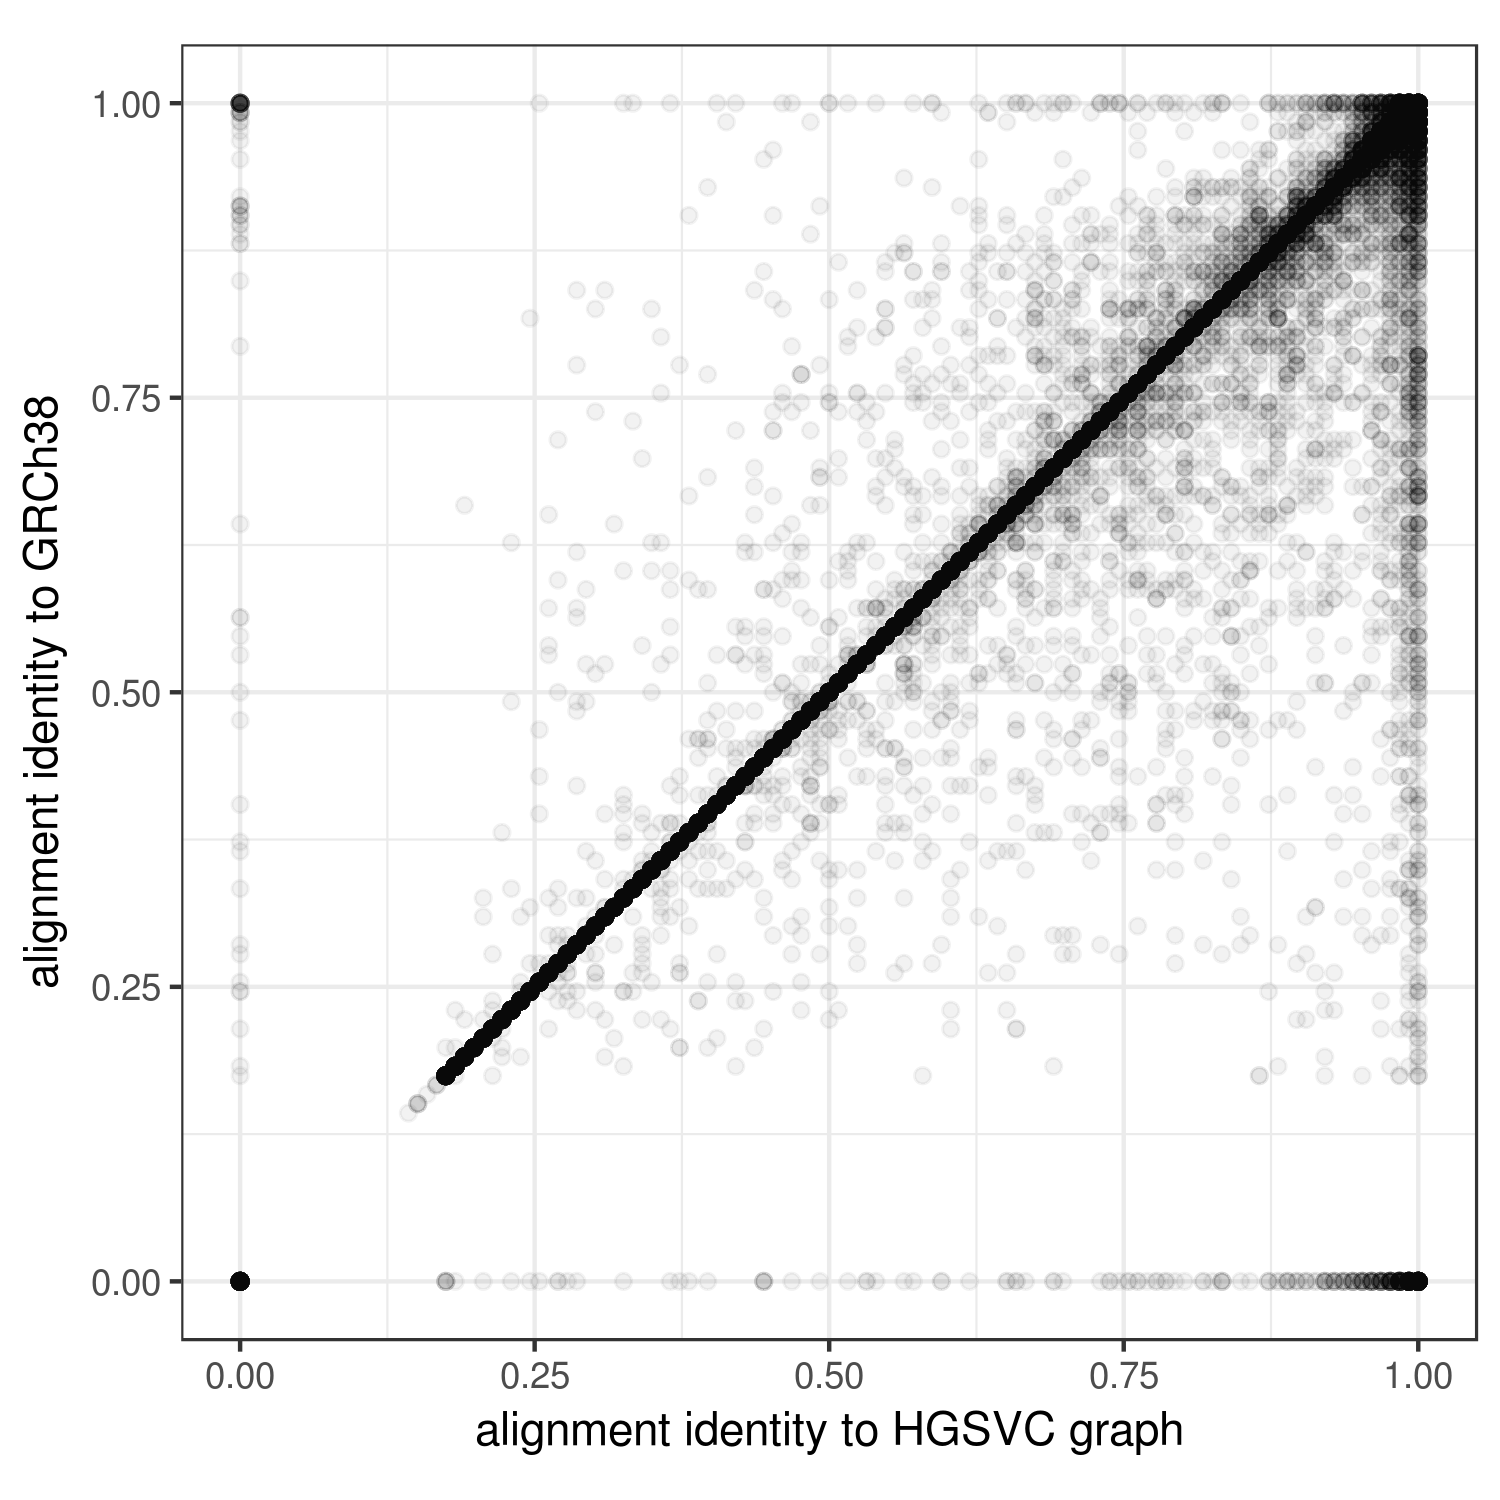
\includegraphics[width=1.0\textwidth]{Chapter3/Figs/NA19240_hg38_vs_HGSVC_scatter.png}
    \caption{NA19240 HGSVC vs. GRCh38}
    \label{subfig:hgsvc_NA19240_scatter}
  \end{subfigure}
  \begin{subfigure}[t]{0.49\textwidth}
    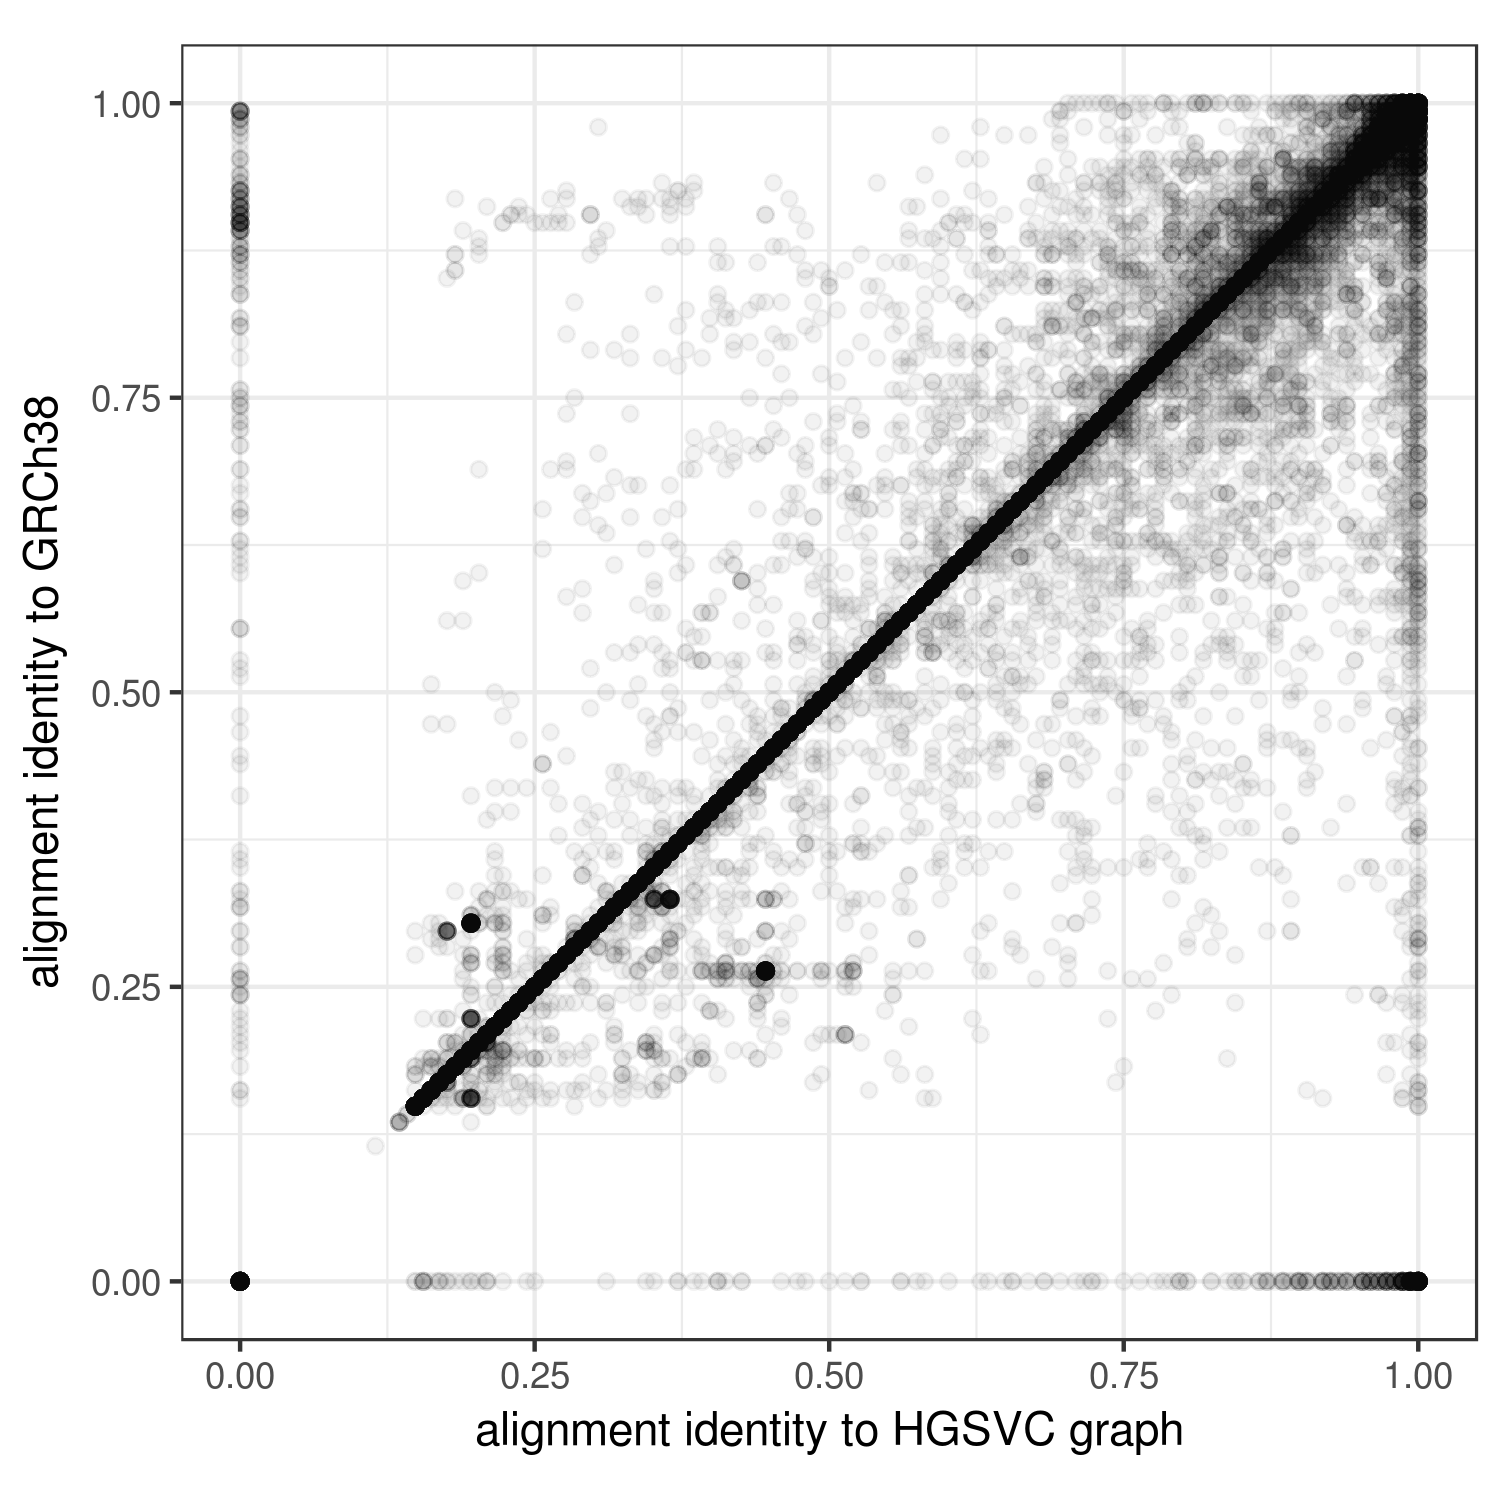
\includegraphics[width=1.0\textwidth]{Chapter3/Figs/NA24385_hg38_vs_HGSVC_scatter.png}
    \caption{NA24385 HGSVC vs. GRCh38}
    \label{subfig:hgsvc_NA24385_scatter}
  \end{subfigure}

  \begin{subfigure}[t]{0.49\textwidth}
    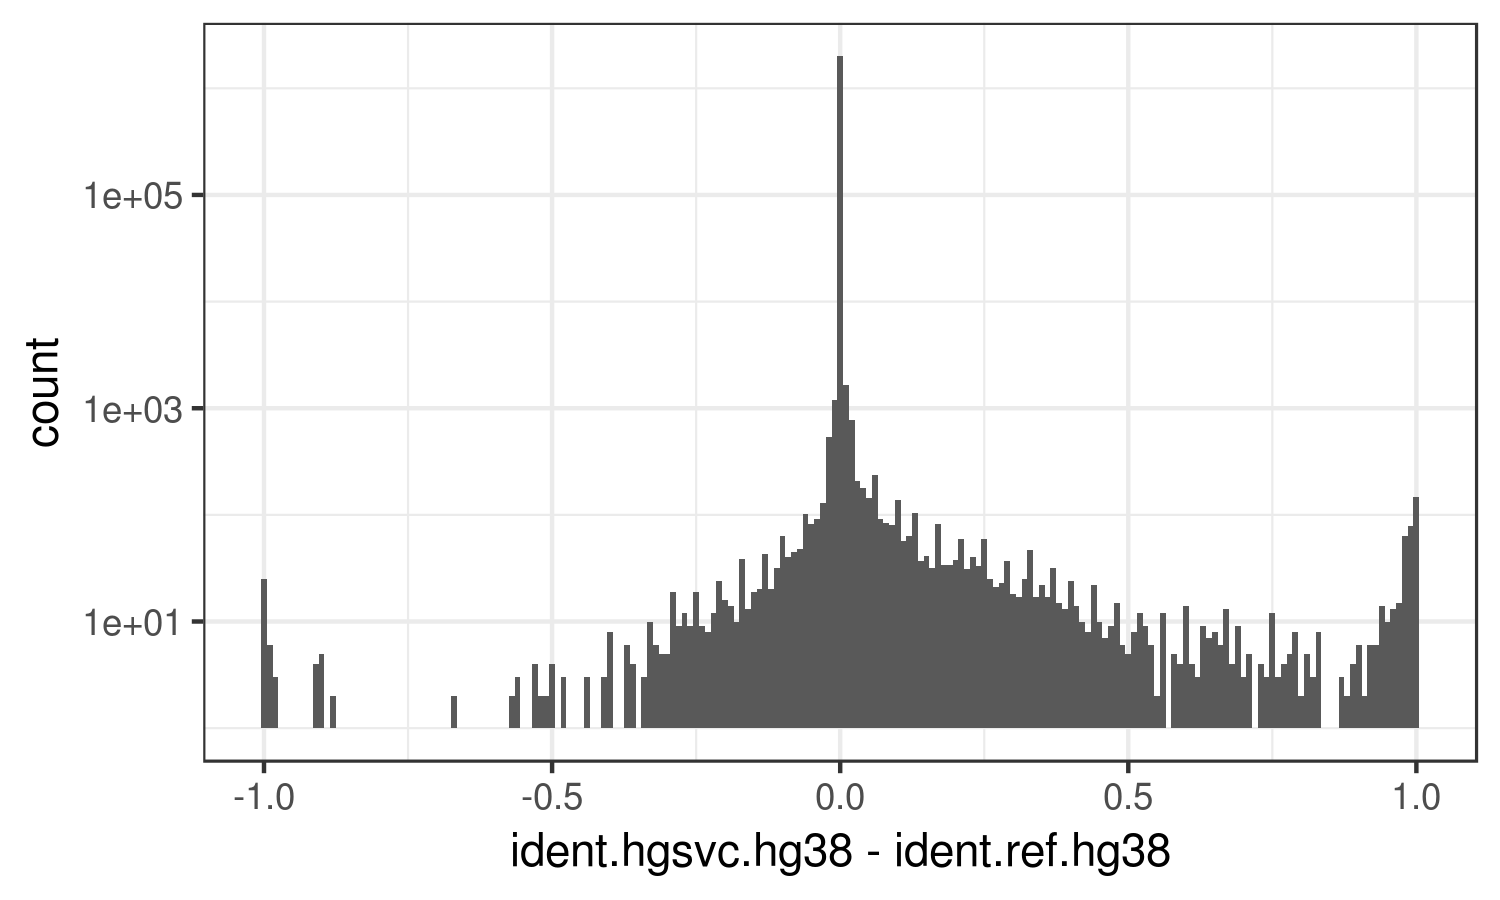
\includegraphics[width=1.0\textwidth]{Chapter3/Figs/NA19240_hg38_vs_HGSVC_hist.png}
    \caption{NA19240 HGSVC - GRCh38}
    \label{subfig:hgsvc_NA19240_hist}
  \end{subfigure}
  \begin{subfigure}[t]{0.49\textwidth}
    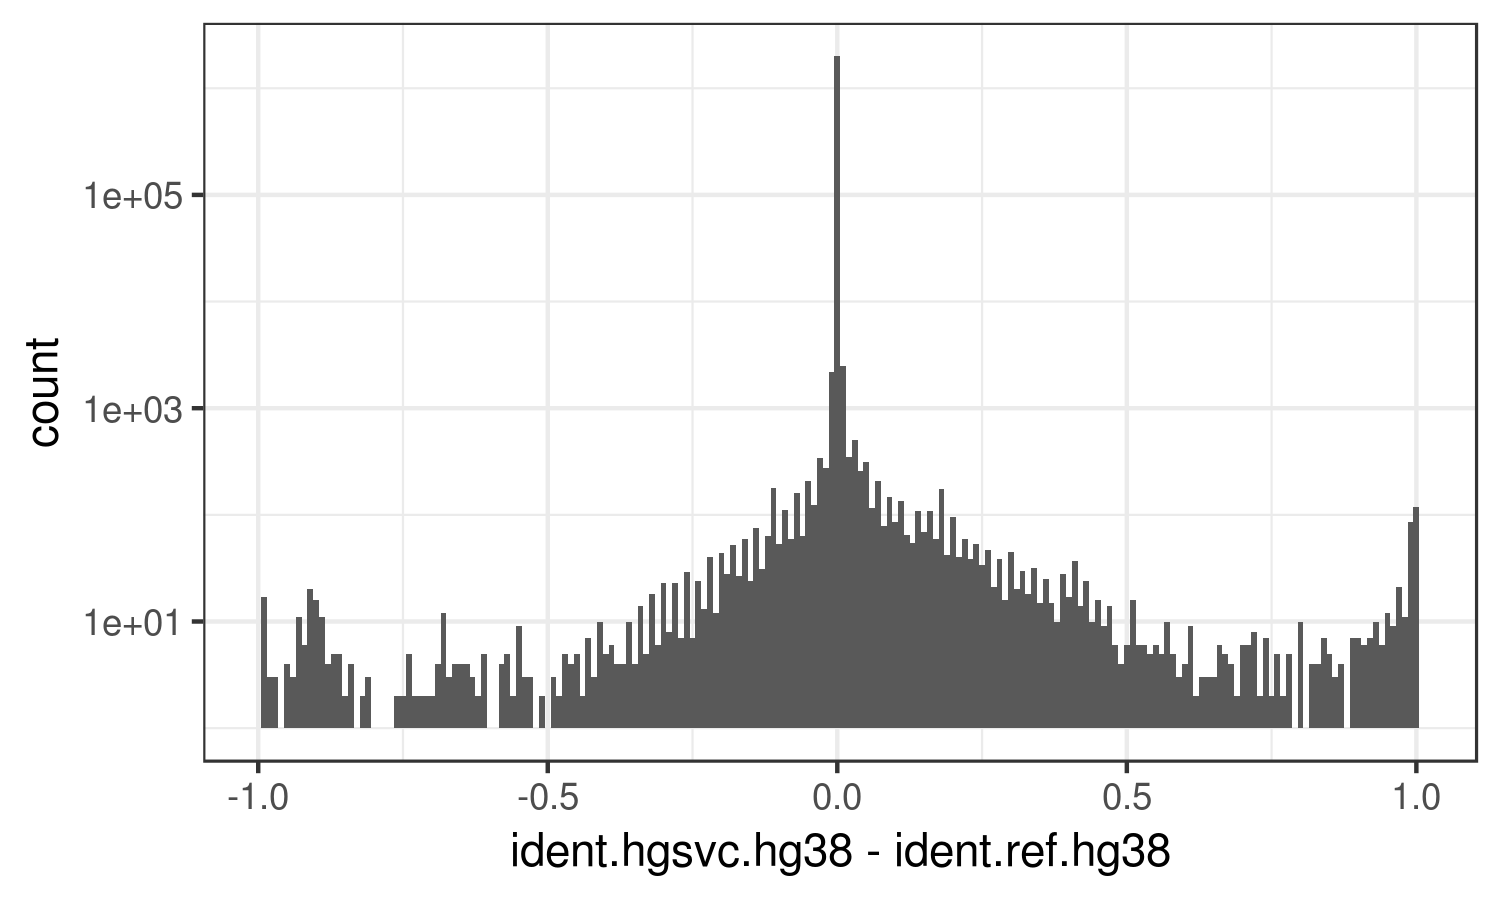
\includegraphics[width=1.0\textwidth]{Chapter3/Figs/NA24385_hg38_vs_HGSVC_hist.png}
    \caption{NA24385 HGSVC - GRCh38}
    \label{subfig:hgsvc_NA24385_hist}
  \end{subfigure}
  \caption[Alignment against the HGSVC graph]{
    1M 2x150bp Illumina read pairs from NA19240 (which is in the HGSVC graph) and NA24385/HG002, which is not, aligned against both the HGSVC graph and the GRCh38 reference, then compared.
    In panels \ref{subfig:hgsvc_NA19240_scatter} and \ref{subfig:hgsvc_NA24385_scatter} the difference in performance is seen by the alignments which have positive identity against the HGSVC graph but 0 identity against the GRCh38 reference.
    Panels \ref{subfig:hgsvc_NA19240_hist} and \ref{subfig:hgsvc_NA24385_hist} are log-scaled histograms of the difference in alignment score.
   }
\label{fig:hgsvc_alignment}
\end{figure}


\subsection{Progressive alignment of human chromosomes}

There are only a handful of truly \emph{de novo} human genome assemblies which achieve near-complete chromosomes, and so a reference-guided variant detection approach has prevailed for the discovery of novel structural variation \cite{fan2017hysa}.
Using the reference-guided assemblies 

\subsection{CHiP-Seq}
%*1p 1h*

This removal of bias is important when mapping functional genomics data such as ChIP-seq data, where allele-specific expression analysis can reveal genetic variation that affects function but is confounded
by reference mapping bias \cite{mcdaniell2010heritable}, especially given that read lengths are typically shorter for these experiments.
We compared mapping with {\tt bwa mem} and {\tt vg} for data set ENCFF000ATK from the ENCODE project \cite{encode2012integrated}, which contains 14.9 million 51-bp ChIP-seq reads for the H3K4me1 histone methylation mark from the NA12878 cell line.
When mapping with bwa the ratio of reference to alternate allele matches at heterozygous sites was 1.20, whereas with vg to the 1000GP graph the ratio was 1.01, effectively eliminating reference bias.


\begin{figure}[htbp!] 
  \centering
  \begin{subfigure}[t]{0.49\textwidth}
    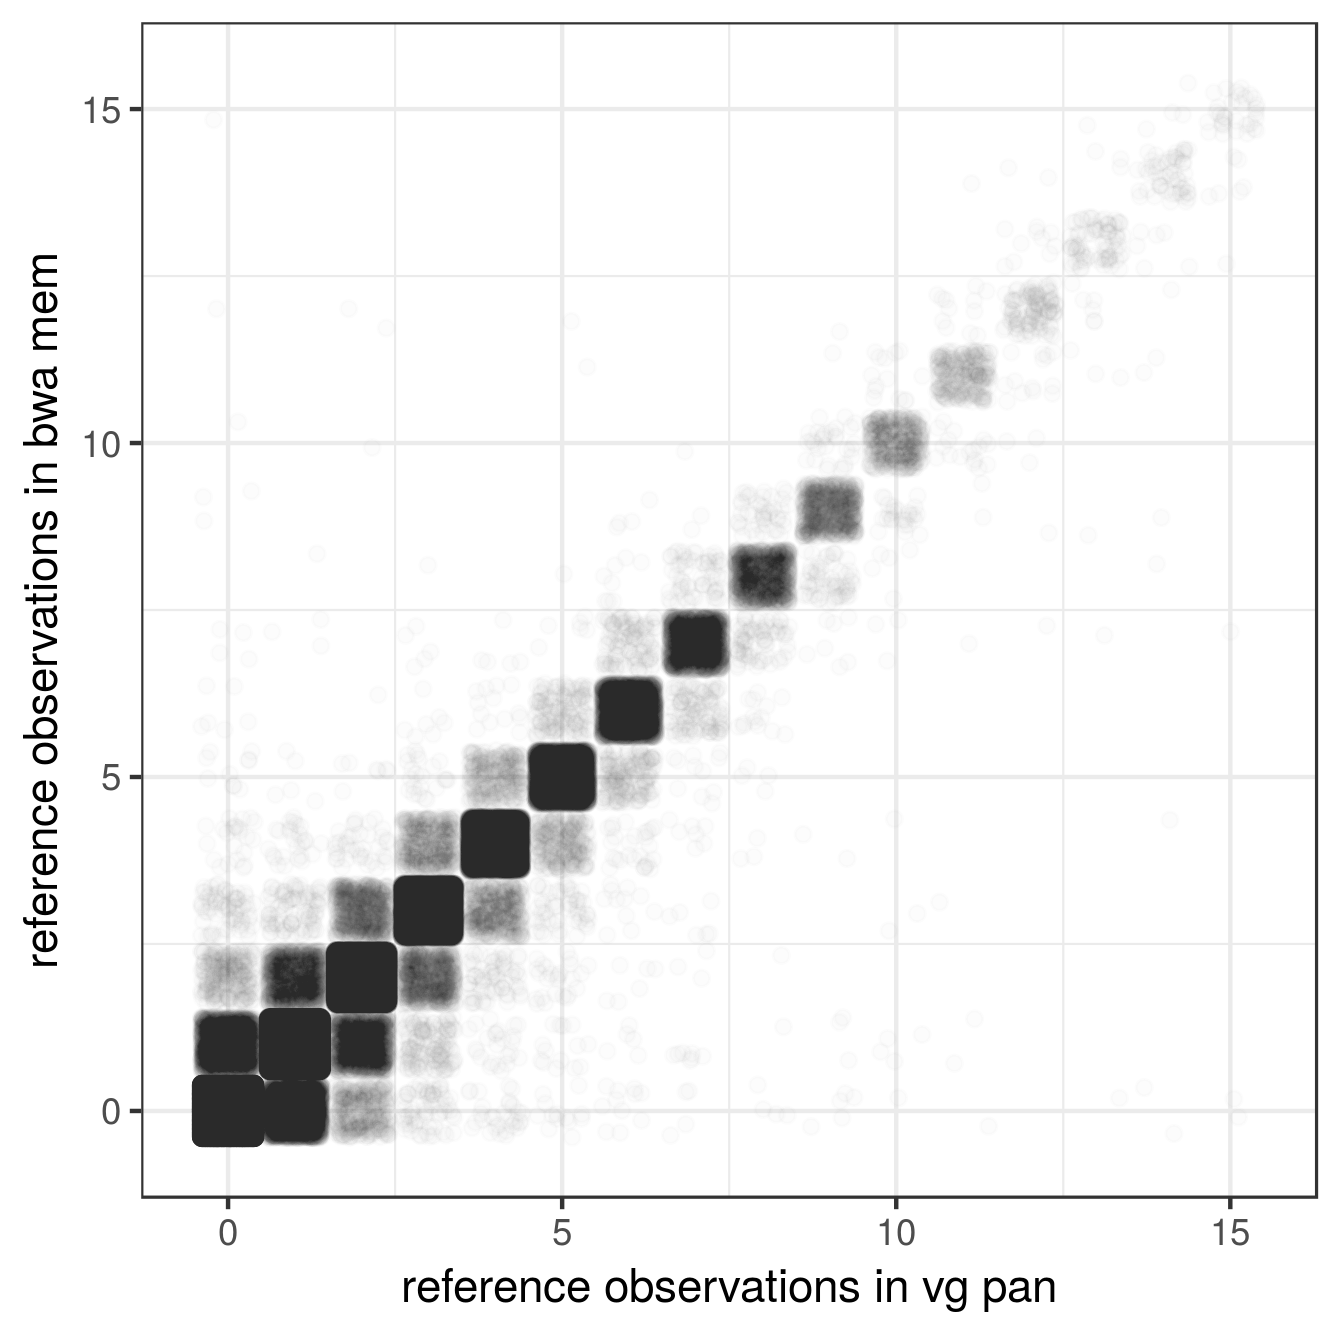
\includegraphics[width=1.0\textwidth]{Chapter3/Figs/ENCFF486KYD_RO_vg_pan_vs_bwa.png}
    \caption{Reference observations}
    \label{subfig:chip_seq_ref_obs}
  \end{subfigure}
  \begin{subfigure}[t]{0.49\textwidth}
    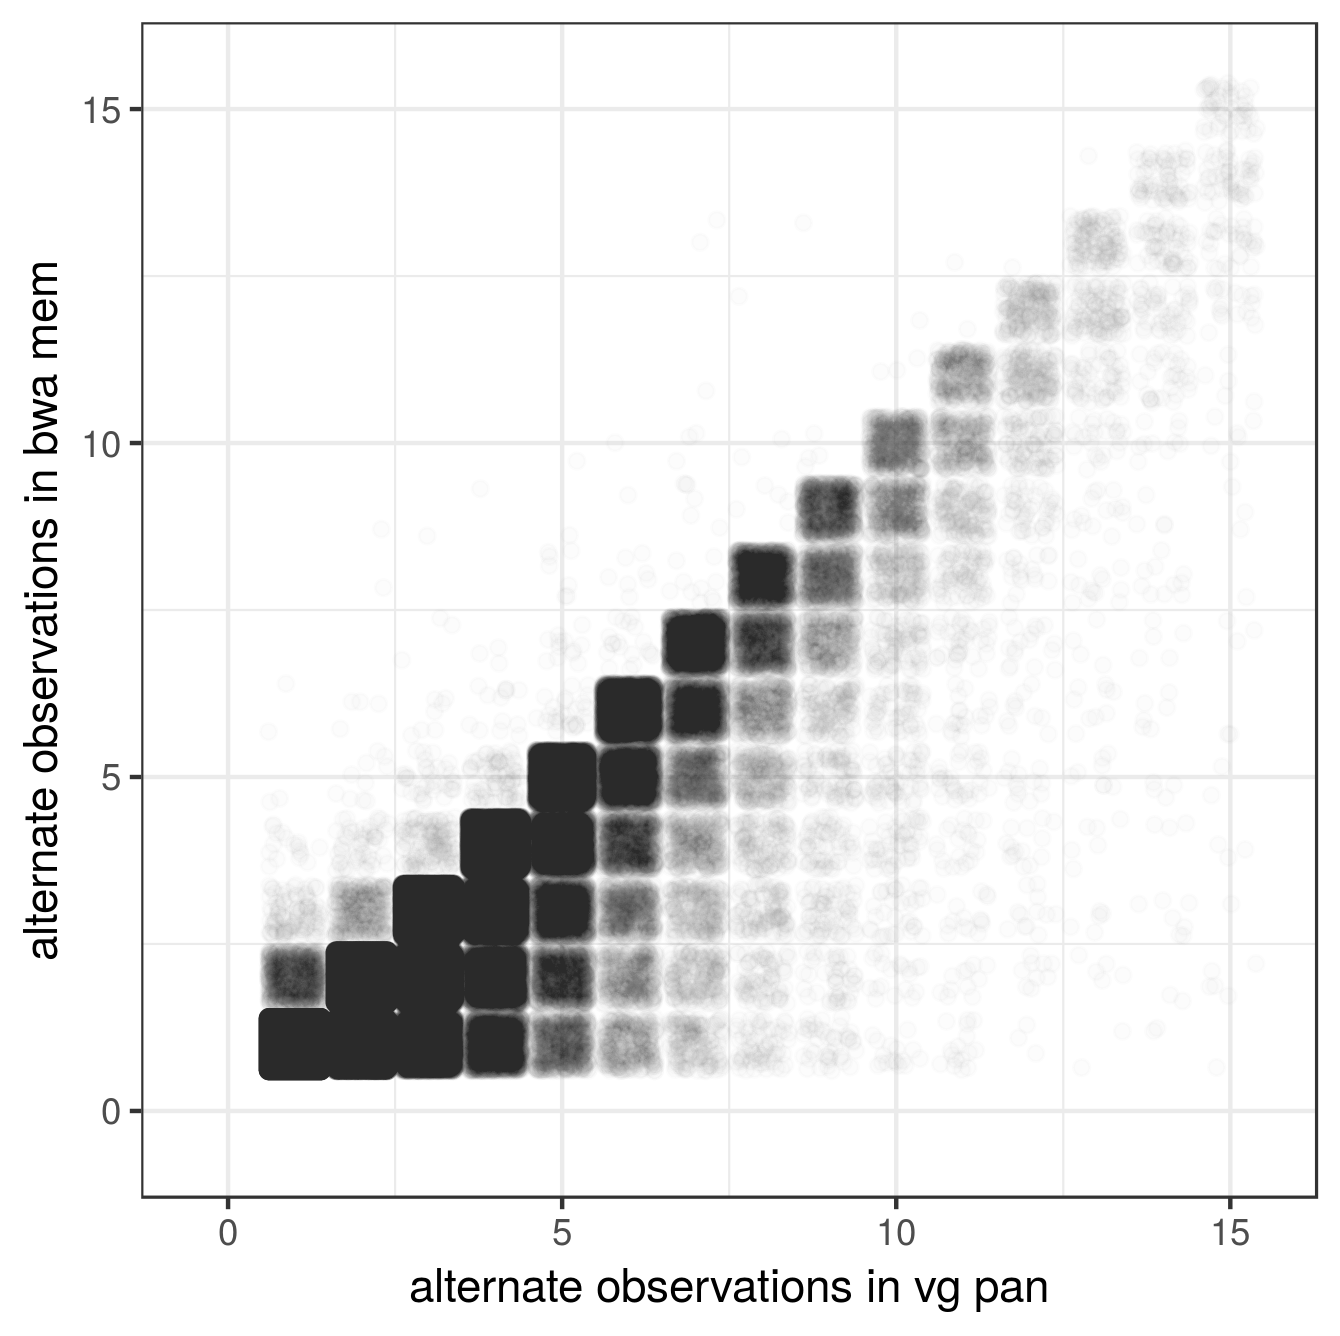
\includegraphics[width=1.0\textwidth]{Chapter3/Figs/ENCFF486KYD_AO_vg_pan_vs_bwa.png}
    \caption{Alternate observations}
    \label{subfig:chip_seq_alt_obs}
  \end{subfigure}
  \caption[Resolving reference bias in 36-bp CHiP-seq]{
    Resolving reference bias in 36-bp CHiP-seq data from ENCODE sample ENCDO115AAA, using CHiP-seq targeting H3K4me1 (experiment ENCFF000ATK).
    We compare the counts of reference-supporting (panel \ref{subfig:chip_seq_ref_obs}) or alternate-supporting (panel \ref{subfig:chip_seq_alt_obs}) alignments between {\tt vg map} and {\tt bwa mem} at sites called as heterozygous in the sample which were also polymorphic in the 1000GP.
   }
\label{fig:chip_seq}
\end{figure}

The effect is dramatically stronger when using 36-bp reads.
To illustrate, I aligned the ultra-short reads from ENCODE experiment ENCSR290YLQ\footnote{\url{https://www.encodeproject.org/experiments/ENCSR290YLQ/}} to the full 1000GP graph using {\tt vg map} and to the GRCh37 reference genome using {\tt bwa mem}.
To simplify analysis, the {\tt vg} mappings were surjected to the GRCh37 reference.
This sample came from an adult donor, and so we have no ``truth'' set as with NA12878, but we can use a subset of sites called as variable using {\tt freebayes} which also are known to be polymorphic in the 1000GP to examine the effect of reference bias.
By plotting the reference and alternate counts obtained from each aligner relative to each other, we can observe the effect of reference bias on a per-site basis\footnote{The longer 51-bp reads are more realistic, but the genome coverage of these sets appears to be lower, and thus it was not possible to generate plots of this kind.}, which can be seen in figure \ref{fig:chip_seq}.
I find that {\tt bwa mem} and {\tt vg map} obtain insignificantly different counts of reference observations at the heterozygous sites (panel \ref{subfig:chip_seq_ref_obs}), but as can be seen in panel \ref{subfig:chip_seq_alt_obs}, aligning to the graph uncovers dramatically more alternate observations at these loci, as is shown by the strong increase in density below the diagonal.
The strength of this effect indicates that small variation will disrupt alignment even with reads of relatively high quality and low error rates.
The issue becomes even more dramatic when we consider data sources with higher error.

\section{Ancient DNA}
%*0.5p 0.5h*
With aDNA, read lengths are limited by the degredation of DNA due to environmental exposure.
Furthermore, degredation causes a high intrinsic error rate.
In combination these issues cause a strong bias against non-reference variation.
This has significant effect on population genetic inference and implications for many aDNA studies.

\subsection{Simulations with human origins panel}
%*1p 2h*

\subsection{Using 1000GP graph for samples from Martiniano et al 2016}
%*2p 4h*

\subsection{Evaluation of a high-coverage Botai sample}
%*2p 4h*


\section{Neoclassical bacterial pangenomics}
%*0.5p 0.5h*

\subsection{E. coli pangenome from illumina reads}
%*2p 4h*

\subsection{Evaluating the core and accessory pangenome}
%*2p 4h*


\section{Metagenomics}
%*0.5p 0.5h*

\subsection{Arctic viral metagenome}
%*2p 1.5h*

\subsection{Human gut microbiome}
%*2p 8h*


\section{RNAseq}
%*0.5p 0.5h*

\subsection{Yeast}
%*1p 2h*

\subsection{C. elegans}
%*2p 5h*

\subsection{Human}
%*2p 12h*


\section{Applications that I contributed to}

% ...
